\documentclass[preprint,12pt,authoryear]{elsarticle}

\usepackage{amsmath,amssymb,amsfonts}
\usepackage{graphicx}
\usepackage{booktabs}
\usepackage{multirow}
\usepackage{array}
\usepackage{tabularx}
\usepackage{xurl}
\usepackage{hyperref}
\usepackage{xcolor}
\usepackage{subcaption}
\usepackage{enumitem}
\usepackage{microtype}
\usepackage{float}
\usepackage{fancyvrb}

\hypersetup{
  colorlinks=true,
  linkcolor=blue,
  citecolor=blue,
  urlcolor=blue,
  pdftitle={Allocation Temperature in Reservoir Computing: Structural Paths, Safe Regions, and Test-Time Sensitivity},
  pdfauthor={Ildefons Magrans de Abril},
  pdfsubject={Allocation temperature, structural paths, validation-safe regions, and test-time sensitivity in reservoir computing},
  pdfkeywords={reservoir computing, echo state networks, allocation temperature, recurrent neural networks, distribution shift, safe operating regions}
}

\setlength{\emergencystretch}{2em}

\journal{Neural Networks}
\biboptions{authoryear,round}

\begin{document}

\begin{frontmatter}

\title{Allocation Temperature in Reservoir Computing: Structural Paths, Safe Regions, and Test-Time Sensitivity}

\author[upc]{Ildefons Magrans de Abril\corref{cor1}}
\ead{ildefons.magrans@upc.edu}
\cortext[cor1]{Corresponding author.}
\address[upc]{Universitat Polit\`ecnica de Catalunya - BarcelonaTech (UPC), Barcelona, Spain}

\begin{abstract}
Reservoir computing fixes recurrent dynamics and typically tunes their scale, update timescale, sparsity, or size. We introduce \emph{allocation temperature}, a structural parameter that redistributes recurrent weight mass across incoming connections while a separate normalization keeps bulk recurrent scale comparable. For the resulting row-wise softmax allocation, row entropy and entropy-equivalent effective support increase monotonically with temperature.

Validation selects a default temperature and a connected region of nearby temperatures with similar performance. Two label-free indicators, prediction dispersion and endpoint spread, quantify how strongly predictions vary across this validation-safe region. They measure structural sensitivity without claiming to identify the lowest-error candidate.

Across controlled time-series and standard reservoir benchmarks, validation-safe regions contain near-optimal held-out temperatures more often than matched same-width intervals. This enrichment persists with a denser 25-point grid and reservoirs of size $N=150$, where containment is $2.16$--$2.86\times$ that of matched controls. Direct improvement within the safe region remains modest, while path-sensitivity indicators correlate $0.41$--$0.58$ with the improvement available inside it. Comparisons with gain, leak rate, and hard sparsity show that allocation temperature defines a distinct structural path but does not universally dominate these controls. In four-split real-data studies, Appliances Energy is a null safe-region-versus-control case, whereas UCI Air Quality gives a positive result.

A final temperature--leak distribution-shift study separates structural opportunity from deployability: target-label upper bounds reveal substantial improvement, whereas a pre-deployment sparse ensemble recovers only part of it and fails under block missingness. Allocation temperature therefore provides an interpretable reservoir-design coordinate and a diagnostic framework for when recurrent allocation matters.
\end{abstract}

\begin{keyword}
reservoir computing \sep echo state networks \sep allocation temperature \sep recurrent neural networks \sep distribution shift \sep safe operating regions
\end{keyword}

\end{frontmatter}

\section{Introduction}
\label{sec:introduction}

Reservoir computing is attractive because it shifts most learning complexity from recurrent training to readout training. Echo state networks and liquid state machines use a fixed recurrent dynamical system to transform input histories into high-dimensional state trajectories, after which a linear or shallow readout can be trained efficiently \citep{jaeger2001echo,maass2002real,lukosevicius2009reservoir}. The recurrent substrate is therefore a central part of the model: it determines how input history is stored, mixed, filtered, and separated before the readout sees it.

Common design choices include spectral radius, input scaling, leak rate, sparsity, reservoir size, and random weight distribution \citep{schrauwen2007overview,lukosevicius2009reservoir,yildiz2012revisiting}. These controls affect different properties. Spectral radius and gain primarily change recurrent amplification, leak rate changes the state-update timescale, and hard sparsity changes the zero/nonzero connectivity pattern. What they do not independently parameterize is how recurrent weight mass is distributed across the connections that remain available. This paper introduces allocation temperature to expose that missing structural degree of freedom.

We summarize this concentration with the row's \emph{effective recurrent support}. The term does not count nonzero edges and does not make a binary decision about whether an edge is present. It is the entropy-equivalent number of equally weighted inputs, $S_{\mathrm{eff}}=\exp(H)$. A sharply concentrated row has low effective support; a diffuse row has high effective support. Because the measure is continuous, values between integers represent graded concentration patterns. This is fundamentally different from hard top-$k$ sparsity, which explicitly removes edges.

We control this graded allocation with a signed row-wise softmax. The parameter $\tau$ is called \emph{allocation temperature} because temperature is also used elsewhere in machine learning to rescale output logits or token probabilities. Here it acts inside the recurrent weight construction, not at the model output. Each row has fixed raw scores $a_{ij}$ and signs $s_{ij}\in\{-1,+1\}$, and allocates recurrent mass according to
\begin{equation}
  p_{ij}(\tau)=\frac{\exp(a_{ij}/\tau)}{\sum_k \exp(a_{ik}/\tau)},
  \qquad
  W_{ij}(\tau)=c(\tau) s_{ij} p_{ij}(\tau),
\end{equation}
where $c(\tau)$ is a global normalization factor chosen to keep the overall recurrent scale comparable across temperatures. This normalization is fixed by a target scale set before the temperature scan, so it is not re-selected separately for each $\tau$. Low allocation temperature concentrates recurrent mass on a few high-score edges. High allocation temperature spreads it more evenly. Allocation temperature therefore defines a smooth structural path through recurrent connectivity while recurrent gain is controlled separately.

The first practical use of this path is conventional: validation can select one temperature as a fixed hyperparameter. The second use is diagnostic. Validation can identify a connected region of nearby temperatures whose performance remains close to the validation optimum. At test time, we can compare the predictions produced by the candidates inside this region. If they agree, changing allocation temperature cannot substantially change the output on that window. If they disagree, the output is sensitive to the structural choice. We call the resulting quantities \emph{path-sensitivity indicators}. They require no test labels. They measure whether changing temperature could matter, not which temperature would be best.

This distinction between \emph{sensitivity} and \emph{target error} is important. Prediction disagreement can be observed without labels, whereas determining which candidate has the lowest target error requires information about the target. The final validation study therefore asks a broader question under distribution shift: how much improvement is available if target labels are allowed retrospectively to choose or combine reservoir structures, how much can be recovered by an ensemble fixed before deployment, and whether unlabeled target-window statistics can predict which candidate will perform best.

This paper makes four main contributions:
\begin{enumerate}[leftmargin=*]
  \item We introduce allocation temperature as a continuous structural control of recurrent weight concentration, separated from recurrent scale, and show analytically that row entropy and effective recurrent support increase monotonically with temperature.
  \item We define a validation-safe structural region and two label-free path-sensitivity indicators that quantify when predictions are sensitive to recurrent allocation without assuming that unlabeled data can identify the lowest-error candidate.
  \item We establish the empirical behavior of this structural axis through controlled comparisons with gain, leak rate, and hard sparsity, standard reservoir benchmarks, two public sensor datasets, and robustness tests over temperature-grid density and reservoir size.
  \item We extend the analysis to distribution shift over a two-dimensional temperature--leak bank, separating the structural improvement available with target labels from what can be recovered by a policy fixed before deployment and identifying conditions under which unlabeled structural adaptation fails.
\end{enumerate}

Allocation temperature is the primary structural contribution. The safe region and path-sensitivity indicators characterize that axis after validation, while the distribution-shift study measures how much broader structural opportunity exists and how difficult it is to exploit without target labels.

The remainder of the paper is organized as follows. Section~\ref{sec:related_work} positions the method relative to reservoir design, adaptive recurrent models, and test-time adaptation. Section~\ref{sec:structural_path} develops the allocation-temperature construction and its entropy interpretation. Section~\ref{sec:methods} describes calibration, uncertainty estimation, and the distribution-shift study. Sections~\ref{sec:core_validation}--\ref{sec:grid_size_robustness} provide the one-dimensional validation, comparison, real-data, and robustness results. Section~\ref{sec:shift_audit_results} presents the final distribution-shift study. Sections~\ref{sec:discussion}--\ref{sec:conclusion} discuss interpretation, limitations, and conclusions. Appendix~\ref{app:repro_map} provides the file-level reproducibility map for the reported experiments.

\section{Related Work}
\label{sec:related_work}

\paragraph{Reservoir computing and echo state networks.}
Reservoir computing trains readouts over fixed recurrent dynamics \citep{jaeger2001echo,maass2002real,lukosevicius2009reservoir}. Much work has studied spectral radius, input scaling, leak rate, sparsity, topology, and state dimension. The present work controls a different property: the continuous concentration of recurrent weight mass within each row while keeping bulk recurrent scale comparable. Allocation temperature changes how sharply a row favors a small subset of incoming connections; a pure gain path multiplies a fixed recurrent shape, and hard sparsity changes the zero/nonzero edge pattern.

\paragraph{Reservoir structure, memory, and dynamics.}
Reservoir performance depends on a balance between memory, nonlinearity, separation, and stability \citep{yildiz2012revisiting}. Hierarchical and multi-timescale reservoirs explicitly combine different dynamical regimes \citep{manneschi2021exploiting}. Recent work has also used entropically regularized optimal transport to create dynamic, input-conditioned inter-assembly coupling in echo-state networks \citep{singh2026ot}. That mechanism computes a doubly stochastic transport plan online and changes routing between reservoir assemblies. Allocation temperature is different: it indexes a static family of row-wise recurrent allocations generated from fixed scores and signs, and validation selects operating points on that family before deployment.

\paragraph{Adaptive continuous-time and hybrid reservoir models.}
A related line of work makes recurrent computation controllable through continuous-time dynamics, neural ordinary differential equations, and adaptive time constants \citep{chen2018neural,hasani2021liquid,hasani2022closed}. Echo State Transformer models combine reservoir memory with attention and include learned softmax-based adaptive leak mechanisms \citep{bendiouis2025est}. These approaches modify online state dynamics or learn state-dependent controls. Allocation temperature addresses a narrower structural question: the recurrent substrate is static for each candidate, and the exposed control axis changes the concentration of recurrent allocation rather than learning a time-varying hidden-state model.

\paragraph{Intrinsic plasticity, adaptive reservoirs, and physical substrates.}
Intrinsic plasticity changes reservoir node response statistics to improve computational usefulness \citep{schrauwen2008improving}. Physical reservoir computing also studies controllable substrates and task-dependent operating points \citep{appeltant2011information,tanaka2019recent,vandoorn2017model}. Allocation-temperature calibration shares the idea that substrate parameters matter, but focuses on a validation-defined structural path and test-time prediction sensitivity rather than online recurrent plasticity.

\paragraph{Test-time adaptation and unlabeled model selection.}
Modern test-time adaptation often uses entropy or consistency to update model parameters at deployment time \citep{wang2021tent,niu2022sentry}. Our path-sensitivity indicators are related in spirit because they are computed on target windows, but they do not update model parameters and do not estimate target error directly. They measure how much predictions vary across a set of structures that was already accepted by validation. Selecting the lowest-error model without target labels is a harder unlabeled risk-estimation problem. The final distribution-shift study evaluates that distinction explicitly inside a reservoir structural bank.

\paragraph{Softmax temperature, attention, and safe optimization.}
Temperature is widely used to control softmax sharpness in probability calibration, attention-like mechanisms, and differentiable categorical relaxations such as the concrete and Gumbel-softmax distributions \citep{guo2017calibration,maddison2017concrete,jang2017categorical}. Graph attention networks normalize learned neighbor scores with a row-wise softmax \citep{velickovic2018graph}, but their coefficients are input-dependent and trained end to end. Here the raw recurrent scores and signs are fixed, and allocation temperature indexes a family of static recurrent substrates rather than calibrating output probabilities or computing sample-dependent attention. The term ``safe region'' also echoes safe optimization and Bayesian optimization \citep{snoek2012practical,sui2015safe}, but here it denotes a validation-defined connected interval over a finite structural path, not a probabilistic constraint set optimized online.

\section{Temperature-Softmax Reservoirs as Structural Paths}
\label{sec:structural_path}


\subsection{Entropy-regularized recurrent allocation}

For a fixed reservoir row $i$, the raw score $a_{ij}$ measures how strongly source unit $j$ is preferred as an incoming recurrent contributor to target unit $i$. Temperature first defines an unsigned row-allocation distribution
\begin{equation}
  p_{ij}(\tau)=\frac{\exp(a_{ij}/\tau)}{\sum_k \exp(a_{ik}/\tau)},\qquad \tau>0,
  \label{eq:row_softmax}
\end{equation}
over candidate recurrent inputs $j$. Thus $p_{ij}(\tau)$ is the fraction of row $i$'s unsigned recurrent mass assigned to source $j$ before the sign and global scale are applied. Given a fixed sign matrix $S\in\{-1,+1\}^{N\times N}$, define the signed allocation matrix
\begin{equation}
  M_{ij}(\tau)=s_{ij}p_{ij}(\tau).
  \label{eq:signed_allocation}
\end{equation}
The final recurrent matrix is
\begin{equation}
  W(\tau)=c(\tau)M(\tau),
  \label{eq:scaled_recurrent_matrix}
\end{equation}
where $c(\tau)>0$ is a scalar chosen after the signed allocation matrix has been constructed. In the experiments we use
\begin{equation}
  c(\tau)=\frac{s_0}{\sqrt{N}\,\operatorname{RMS}(M(\tau))},
  \label{eq:scale_normalization}
\end{equation}
where $\operatorname{RMS}(M)=\sqrt{N^{-2}\sum_{ij}M_{ij}^2}$ is the element-wise RMS. This convention makes the element-wise RMS of $W(\tau)$ equal to $s_0/\sqrt{N}$, giving a comparable bulk recurrent scale across temperatures and reservoir sizes. The target scale $s_0$ is fixed before scanning temperature; in all reported temperature-path experiments we set $s_0=1$ unless otherwise stated. In principle, $s_0$ could be selected by validation like an ordinary recurrent-gain hyperparameter, but it is not re-selected across the temperature grid. This separation is central: $p_i(\tau)$ controls row-wise allocation entropy and effective support, while $c(\tau)$ keeps the overall recurrent scale comparable across temperatures. The separate gain-path baseline deliberately varies this global scale to test whether temperature effects reduce to ordinary gain effects.

The row-softmax in Eq.~\eqref{eq:row_softmax} is the standard solution of an entropy-regularized linear allocation problem:
\begin{equation}
  p_i(\tau)=\arg\max_{p\in\Delta}\left[\sum_j p_j a_{ij}+\tau H(p)\right],
  \label{eq:entropy_regularized_allocation}
\end{equation}
where $H(p)=-\sum_j p_j\log p_j$ and $\Delta=\{p:p_j\ge 0,\sum_j p_j=1\}$ is the probability simplex. The score term rewards allocating mass to high-score recurrent inputs; the entropy term rewards spreading mass across inputs. This is the standard Gibbs or maximum-entropy construction: temperature sets the strength of the entropy term relative to the score term \citep{jaynes1957information}. A short derivation is given in Appendix~\ref{app:derivations}. As $\tau\rightarrow 0$, the distribution concentrates on the largest raw score. As $\tau\rightarrow\infty$, it approaches the uniform distribution.

\subsection{Monotonic effective support and concentration}

Let $H_i(\tau)=-\sum_j p_{ij}(\tau)\log p_{ij}(\tau)$ denote the entropy of row $i$'s unsigned allocation. Writing $Z_i(\tau)=\sum_j\exp(a_{ij}/\tau)$, define the allocation-weighted mean raw score
\[
  \mu_i(\tau)
  \equiv \mathbb{E}_{J\sim p_i(\tau)}[a_{iJ}]
  =\sum_j p_{ij}(\tau)a_{ij}.
\]
Here the scores $a_{ij}$ are fixed numbers; only the weights $p_{ij}(\tau)$ assigned to them change with temperature. With this notation, the entropy can be expressed as
\begin{equation}
  H_i(\tau)=\log Z_i(\tau)-\frac{\mu_i(\tau)}{\tau}.
  \label{eq:entropy_identity}
\end{equation}
Differentiating this expression yields
\begin{equation}
  \frac{d H_i}{d\tau}
  =\frac{\operatorname{Var}_{p_i(\tau)}(a_i)}{\tau^3}\ge 0,
  \label{eq:entropy_derivative}
\end{equation}
where
\[
  \operatorname{Var}_{p_i(\tau)}(a_i)
  =\sum_j p_{ij}(\tau)\bigl(a_{ij}-\mu_i(\tau)\bigr)^2.
\]
Thus entropy increases monotonically with temperature, except in the degenerate case where all row scores are equal. Appendix~\ref{app:derivations} expands Eq.~\eqref{eq:entropy_identity} directly from the softmax definition and then derives Eq.~\eqref{eq:entropy_derivative}; the result assumes that the raw scores $a_{ij}$ are fixed while $\tau$ varies.

For interpretability, we also report the effective support
\begin{equation}
  S_{\mathrm{eff},i}(\tau)=\exp(H_i(\tau)).
  \label{eq:effective_support}
\end{equation}
This quantity is the entropy-equivalent number of equally weighted recurrent inputs. It is a continuous measure of concentration, not a literal count of active or nonzero connections; it expresses the same entropy in units that are easier to interpret. If a row spreads mass uniformly over exactly $k$ inputs, then $H_i=\log k$ and $S_{\mathrm{eff},i}=k$. Equation~\ref{eq:entropy_derivative} implies that $S_{\mathrm{eff},i}(\tau)$ also increases monotonically with $\tau$ because the exponential is monotone. This result is independent of downstream task performance: increasing temperature has a structural effect before any readout is trained.

The monotonicity statement concerns the allocation distribution $p_i(\tau)$, not the post-normalized matrix scale. The scalar $c(\tau)$ in Eq.~\eqref{eq:scale_normalization} affects the global magnitude of $W(\tau)$ but not the row entropy of $p_i(\tau)$. This is why temperature is separated from a simple gain path: changing gain multiplies a fixed recurrent shape, whereas changing temperature alters which recurrent inputs receive mass while the overall scale is controlled separately.

\subsection{From structural control to empirical calibration}

The monotonicity result identifies what temperature controls at the level of recurrent allocation: increasing $\tau$ makes each row distribution less concentrated and increases its effective support. It does not determine the consequences for the complete reservoir dynamics. Although the normalization $c(\tau)$ keeps the bulk recurrent scale comparable, redistributing recurrent mass changes the signed matrix $W(\tau)$ and can affect spectral radius, short-term amplification, contractivity and echo-state behavior, memory, state separation, nonlinear saturation, and ultimately task performance \citep{jaeger2001echo,lukosevicius2009reservoir,yildiz2012revisiting}. Temperature should therefore be understood as a structural allocation axis that is distinct from, but not dynamically independent of, gain and leak-rate controls. We consequently do not infer a useful operating regime from allocation entropy alone. Instead, spectral-radius variation is audited as one possible dynamical confound, while validation performance identifies the candidate temperatures that remain empirically plausible operating points.

For a fixed input sequence $u_t$, reservoir dynamics are
\begin{equation}
  x_{t+1}^{(\tau)}=\tanh\left(W(\tau)x_t^{(\tau)}+W_{\mathrm{in}}u_t\right),
  \qquad
  \widehat y_t^{(\tau)}=r_\tau(x_t^{(\tau)}),
\end{equation}
where $r_\tau$ is the trained readout for temperature $\tau$. The reservoir state is obtained by iterating this recurrence sequentially through the input series. In the experiments, the state is initialized at zero and an initial washout prefix is discarded before readout fitting or evaluation, reducing dependence on the arbitrary initial condition. No fixed-point solution is computed separately for each sample; $x_t^{(\tau)}$ is the state reached after processing the input history up to time $t$. Since $W(\tau)$ varies smoothly for $\tau>0$, the state and prediction traces define a path over allocation temperature. This prediction path becomes operationally meaningful after validation identifies which temperatures remain plausible operating points for the task.

\begin{figure}[t]
\centering
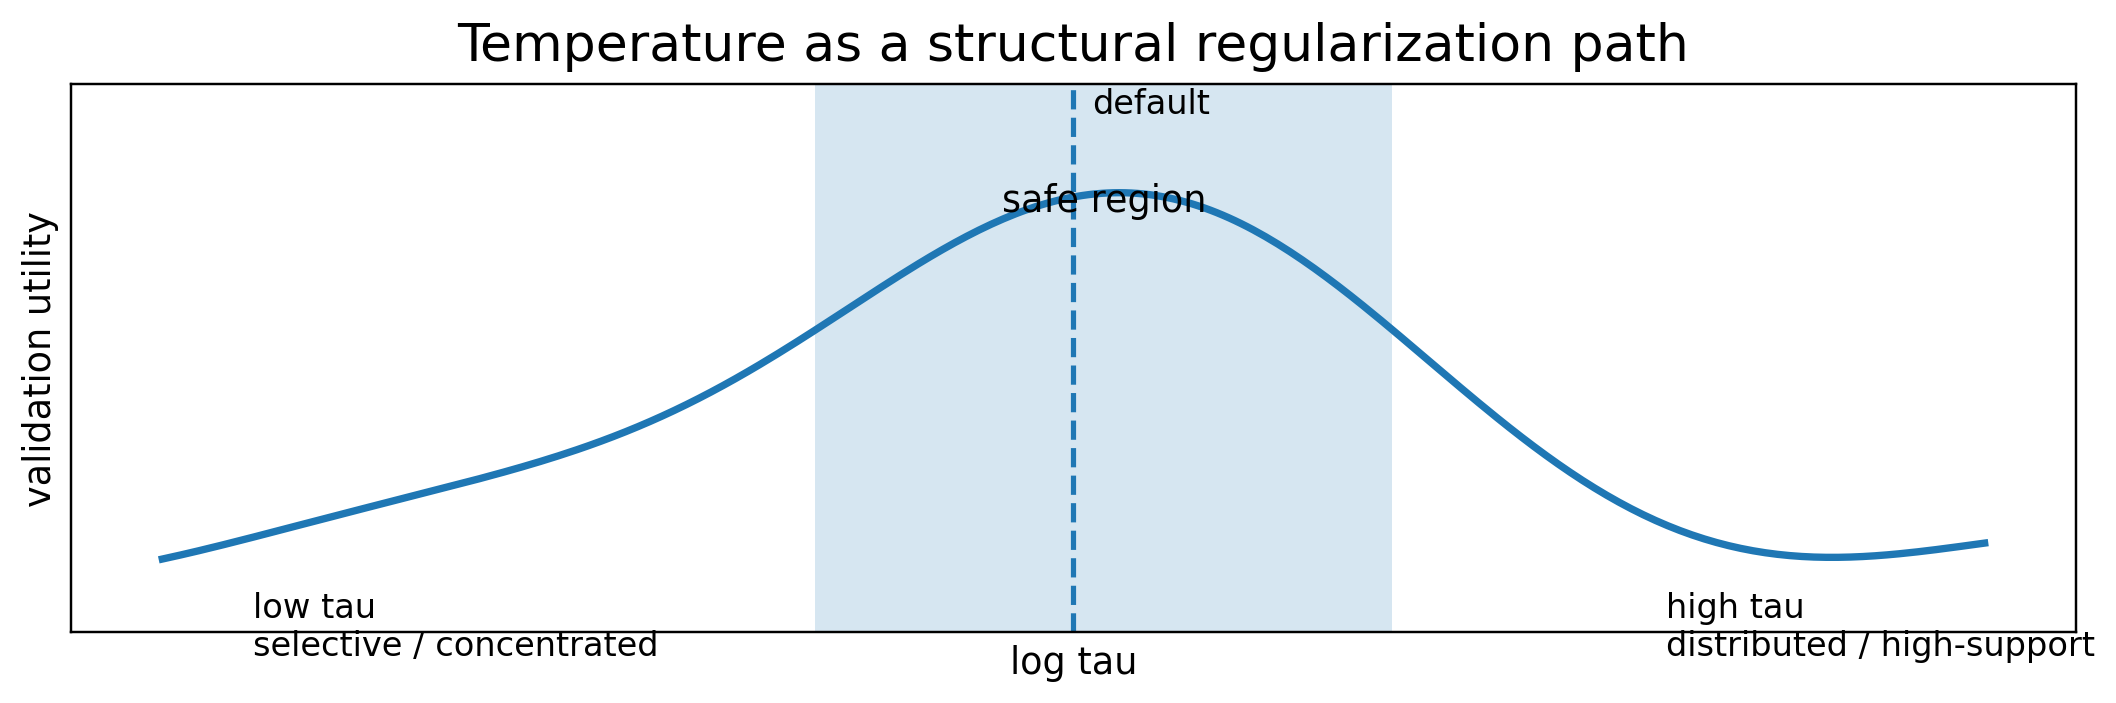
\includegraphics[width=0.78\textwidth]{fig1_conceptual_path.png}
\caption{Conceptual view. Temperature defines a structural path over recurrent allocation. Validation selects a default temperature and a connected safe region around it. Test-time indicators measure whether predictions vary meaningfully inside this safe region.}
\label{fig:conceptual_path}
\end{figure}

Let $U_{\mathrm{val}}(\tau)=-\mathcal L_{\mathrm{val}}(\tau)$ denote validation utility. We choose
\begin{equation}
  \tau_{\mathrm{default}}=\arg\max_{\tau\in\mathcal T}U_{\mathrm{val}}(\tau),
\end{equation}
where $\mathcal T$ is the discrete grid of tested temperatures. The validation-safe region is the connected component containing $\tau_{\mathrm{default}}$ of the validation superlevel set
\begin{equation}
  \mathcal T_{\mathrm{safe}}=
  \left\{\tau\in\mathcal T:
  U_{\mathrm{val}}(\tau)\ge U_{\mathrm{val}}(\tau_{\mathrm{default}})-\epsilon
  \right\}.
  \label{eq:safe_region}
\end{equation}
The connected-component requirement prevents disjoint validation peaks from being merged into a single operating region. Thus the safe region is not a dynamical guarantee; it is an empirical, validation-defined subset of the structural path. Temperatures outside this set are not used for test-time movement.

\subsection{Possible movement gain and path-sensitivity indicators}

The best-safe gain on a labelled test window $w$ is
\begin{equation}
  G_{\mathrm{safe}}(w) =
  \max_{\tau\in\mathcal{T}_{\mathrm{safe}}}
  U_{\mathrm{test},w}(\tau)
  - U_{\mathrm{test},w}(\tau_{\mathrm{default}}).
\end{equation}
This quantity is not available at deployment because it requires labels. It is used only during validation to ask whether changing temperature inside the calibrated safe region could have helped on that window.

Two label-free path-sensitivity indicators measure whether predictions change enough across the safe region for temperature choice to matter. The first indicator is prediction dispersion across the validation-safe temperatures:
\begin{equation}
  D_{\mathrm{safe}}(w)=
  \frac{1}{|w|}\sum_{t\in w}
  \operatorname{Std}_{\tau\in\mathcal{T}_{\mathrm{safe}}}
  \left(\widehat y_t^{(\tau)}\right),
\end{equation}
where $\operatorname{Std}$ denotes the standard deviation across the predictions produced by the candidate temperatures in $\mathcal{T}_{\mathrm{safe}}$ at the same time point. The second indicator is the low/high anchor spread,
\begin{equation}
  A_{\mathrm{LH}}(w)=
  \operatorname{RMSE}\left(
  \widehat y_{w}^{(\tau_{\mathrm{low}})},
  \widehat y_{w}^{(\tau_{\mathrm{high}})}
  \right),
\end{equation}
where $\tau_{\mathrm{low}}$ and $\tau_{\mathrm{high}}$ are the endpoints of $\mathcal{T}_{\mathrm{safe}}$. Low dispersion implies that all safe temperatures produce similar predictions, so changing temperature inside the safe region cannot substantially change the output. High dispersion does not guarantee improvement, but it shows that a labelled choice among the safe temperatures could change the prediction enough to matter.

The interpretation is direct. If all accepted operating points produce nearly identical predictions on a window, choosing among them cannot materially change the output. If the predictions differ, the model is sensitive to the structural choice on that window. This is why the indicators are evaluated as signals of possible improvement rather than as automatic model selectors.

\section{Methods}
\label{sec:methods}

The experimental design follows the same sequence used at deployment: construct comparable reservoir candidates, fit one readout per candidate, use validation data to select an operating region, evaluate that region on held-out data, and estimate uncertainty at the level of independent tasks, trials, splits, or reservoir substrates.

\subsection{Constructing and evaluating the reservoir path}
\label{sec:path_construction_methods}

All one-dimensional temperature experiments use the signed row-wise softmax construction from Section~\ref{sec:structural_path}. For a given reservoir instance, the raw scores, signs, input weights, and data split remain unchanged while allocation temperature varies. The normalization factor $c(\tau)$ is recomputed from Eq.~\eqref{eq:scale_normalization} so that the bulk recurrent scale remains comparable across temperatures. With the element-wise RMS convention used here, $s_0=1$ gives recurrent entries with RMS $1/\sqrt{N}$ after normalization.

The robustness implementation makes the random substrate explicit. Off-diagonal raw scores are sampled independently from a standard normal distribution, recurrent signs are sampled independently with equal probability from $\{-1,+1\}$, self-connections are excluded, and input weights are sampled uniformly within the configured input-scale interval. The same raw-score matrix, sign matrix, and input matrix are then reused for every temperature in a given trial. The released experiment files specify the corresponding seeds and task-specific input scales.

Each candidate temperature defines a different recurrent matrix and therefore a different state trajectory. A separate ridge-regression readout is fitted for every candidate using the same training split, and all candidates are evaluated on the same validation and test splits. Reservoir states are generated sequentially from a zero initial state. An initial washout segment is discarded before fitting or scoring. Performance is measured by normalized root mean squared error (NRMSE), with normalization by the target standard deviation. Utility is defined as negative NRMSE so that larger utility is better.

An NRMSE improvement of $0.005$ means that RMSE decreases by $0.5\%$ of one target standard deviation. We therefore report both the gain available inside the validation-safe region and the corresponding absolute NRMSE values where they are available. This distinguishes modest improvements obtained by choosing among already accepted temperatures from the larger upper bounds obtained by searching or combining a broader structural bank.

\subsection{Selecting a validation-safe region and computing test-time indicators}
\label{sec:safe_region_methods}

Training and validation determine the operating choices that are available before test targets are known. The finite set $\mathcal A=\{a_1,\ldots,a_K\}$ denotes the candidate values along a one-dimensional reservoir path. For allocation temperature, $a_k=\tau_k$. The same calibration procedure is also applied to three comparison paths: recurrent gain, leak rate, and hard top-$k$ sparsity. The gain path multiplies a fixed recurrent matrix. The leak-rate path uses $x_{t+1}=(1-\alpha_k)x_t+\alpha_k\tanh(Wx_t+W_{\mathrm{in}}u_t)$. The hard-sparsity path retains the top-$k$ scored recurrent inputs per row before scale normalization.

The absolute tolerance $\epsilon$ in Eq.~\eqref{eq:safe_region} is obtained from a relative tolerance by
\begin{equation}
  \epsilon = \max\!\left\{\epsilon_{\mathrm{abs}},\;\epsilon_{\mathrm{rel}}\left[\max_{a\in\mathcal A}U_{\mathrm{val}}(a)-\min_{a\in\mathcal A}U_{\mathrm{val}}(a)\right]\right\}.
  \label{eq:tolerance_rule}
\end{equation}
Unless otherwise stated, $\epsilon_{\mathrm{rel}}=0.10$. The absolute floor follows the frozen protocol of each study: $\epsilon_{\mathrm{abs}}=0.005$ in the controlled synthetic/path experiments and $\epsilon_{\mathrm{abs}}=0.002$ in the two real-world sensor studies. The relative term scales the tolerance with the observed validation range, while the absolute floor avoids an unrealistically narrow threshold on nearly flat validation curves. Each study uses the same resulting numerical tolerance retrospectively when identifying near-optimal test candidates. In tolerance-sensitivity analyses, the study-specific $\epsilon_{\mathrm{abs}}$ remains fixed and $\epsilon_{\mathrm{rel}}$ is varied.

\begin{center}
\fbox{\begin{minipage}{0.94\textwidth}
\textbf{Algorithm 1: Calibration and test-time path-sensitivity workflow}\vspace{0.4em}

\textbf{Input:} a reservoir path $\{W(a):a\in\mathcal A\}$, training and validation data, a test stream, and tolerance $\epsilon$.\vspace{0.25em}

\begin{enumerate}[leftmargin=*]
\item Train one readout for every candidate operating point using the training data.
\item Measure validation performance at every candidate point.
\item Choose the validation-best point $a_{\mathrm{default}}$ as the default operating point.
\item Retain the connected neighboring candidates whose validation utility is within $\epsilon$ of the default. This is the validation-safe region $\mathcal A_{\mathrm{safe}}$.
\item Record the low and high endpoints of the safe region.
\item On each test window, compare predictions across the safe candidates. Compute prediction dispersion and low/high endpoint spread.
\item Use these quantities to report how sensitive the prediction is to structural choices that were already accepted by validation. Target labels are required to determine which candidate has the lowest test error.
\end{enumerate}
\end{minipage}}
\end{center}

For retrospective evaluation, we identify the best test candidate on the tested grid and a near-optimal set consisting of candidates within the fixed utility tolerance of that best point. These labels are used only to evaluate whether validation selected a useful part of the path.

\subsection{Validation questions}
\label{sec:validation_plan}

The experiments address five validation questions, each developed in a dedicated results section.

\begin{enumerate}[leftmargin=*]
\item \textbf{Does the validation-safe region transfer to held-out data?} Section~\ref{sec:core_validation} measures exact and near-optimal containment, improvement over the validation-selected default, and comparisons with same-width control intervals. Table~\ref{tab:validation_summary} and Fig.~\ref{fig:m19_validation} summarize the main results.

\item \textbf{Do prediction differences across safe temperatures identify windows with more available improvement?} Section~\ref{sec:core_validation} relates prediction dispersion and endpoint spread to the improvement that could be obtained with labels, and then evaluates the same idea on standard reservoir tasks. Figure~\ref{fig:indicator_reliability} and Fig.~\ref{fig:standard_boundary} show these results.

\item \textbf{Is allocation temperature distinct from established reservoir controls, and does the behavior transfer to measured sensor data?} Section~\ref{sec:path_ablation} compares allocation temperature with gain, leak rate, and hard sparsity. Section~\ref{sec:real_world} evaluates Appliances Energy Prediction and UCI Air Quality \citep{candanedo2017accurate,devito2008field}. Tables~\ref{tab:path_ablation} and \ref{tab:real_world} and Fig.~\ref{fig:path_ablation} contain the corresponding results.

\item \textbf{Are the conclusions sensitive to the safe-region tolerance, spectral-radius changes, grid density, or reservoir size?} Section~\ref{sec:additional_validation} examines safe-region width, tolerance, and structural confounds. Section~\ref{sec:grid_size_robustness} independently changes temperature-grid density and reservoir size. Tables~\ref{tab:m21_safe_width}--\ref{tab:m23_absolute_performance} report the numerical results.

\item \textbf{How much structural improvement is available under distribution shift, and how much can be recovered without target labels?} Section~\ref{sec:shift_audit_results} compares a fixed structure chosen before deployment, a sparse ensemble fitted on pre-deployment conditions, an unlabeled error-prediction model, and an upper-bound ensemble fitted retrospectively with target labels. Tables~\ref{tab:shift_task_results} and \ref{tab:shift_family_results} summarize the outcomes.
\end{enumerate}

Appendix~\ref{app:repro_map} provides a compact mapping from each results section, table, and figure to the corresponding computational notebook and released artifacts.

\subsection{How uncertainty is estimated}
\label{sec:uncertainty_methods}

We report 95\% bootstrap confidence intervals around mean gains and other summary statistics. For each analysis, 30,000 bootstrap samples are generated, the statistic is recomputed for each sample, and the 2.5th and 97.5th percentiles form the interval.

The resampling unit matches the independent unit of the experiment. When an analysis produces one result per independent task, trial, or split, those units are resampled directly. When many overlapping test windows come from the same task and reservoir trial, all windows from a task--trial run are kept together and complete runs are resampled. This cluster bootstrap preserves the dependence among windows that share the same reservoir instance and test sequence.

The grid-and-size robustness study contains four tasks and four trials per task, giving up to 16 task--trial clusters for the continuous indicator analysis. Some clusters are omitted from that specific analysis when the safe region contains only one candidate because prediction variation across a single candidate is undefined. In the distribution-shift study, each task has three independent reservoir substrates. We therefore report the observed task means in Table~\ref{tab:shift_task_results} and avoid emphasizing task-specific resampled confidence intervals. For the comparison across shift types, the resampling unit is the task--substrate pair, giving nine independent clusters; all windows from a selected cluster are kept together. The reported percentile intervals summarize uncertainty across this finite set of clusters.

\subsection{Distribution-shift study}
\label{sec:shift_audit_methods}

The final validation study asks whether the structural degrees of freedom revealed by allocation temperature remain useful when the test distribution changes. It deliberately broadens the structural candidate set from the one-dimensional temperature path to a two-dimensional temperature--leak grid. This makes it possible to separate two questions: how much improvement is available in principle, and how much of that improvement can be obtained without target labels. The corresponding results are reported in Section~\ref{sec:shift_audit_results}.

\paragraph{Candidate bank and forecasting tasks.}
The study uses NARMA10, Mackey--Glass, and Lorenz-$x$. Each task is evaluated with three independent reservoir substrates of size $N=45$. For each task and substrate, the candidate bank is
\begin{equation}
  \Theta_{\mathrm{global}}
  =\{\tau_1,\ldots,\tau_{11}\}\times\{\alpha_1,\ldots,\alpha_{11}\},
\end{equation}
where allocation temperature is logarithmically spaced from $0.08$ to $3.50$ and leak rate is linearly spaced from $0.10$ to $1.00$. The 121 candidates share the same raw-score and sign substrate. Each candidate has its own ridge readout trained on the clean training sequence.

\paragraph{Conditions available before deployment.}
The policies that do not use target labels are fitted using a set of pre-deployment conditions. These include clean operation, two levels of additive AR(1) input noise, and two levels of multiplicative gain drift. AR(1) noise is temporally correlated input noise rather than independent white noise. Gain drift changes the input amplitude multiplicatively. Six episodes are generated for each of these conditions.

\paragraph{Held-out test shifts.}
Evaluation uses shift conditions that are not used to fit the deployable policies: stronger additive AR(1) noise, two levels of additive offset drift, and two levels of block missingness. Block missingness removes contiguous portions of the input rather than merely perturbing their values. Four episodes are generated for each held-out condition. Every episode contains a 180-step context segment followed by a 180-step segment on which NRMSE is scored after washout. Target values from these held-out segments are used only for retrospective evaluation and for the explicitly label-informed upper bound described below.

\paragraph{Policies compared.}
Four alternatives are evaluated within the same candidate set.
\begin{enumerate}[leftmargin=*]
\item \textbf{Fixed structure chosen before deployment.} One temperature--leak candidate is selected by its mean error across the pre-deployment conditions. It is then used unchanged on held-out shifts.
\item \textbf{Sparse ensemble fitted before deployment.} Up to five candidate predictions are combined with nonnegative weights that sum to one. The weights are fitted only on the pre-deployment conditions:
\begin{equation}
  \widehat y^{\mathrm{pre}}_w
  =\sum_{\theta\in\Theta_q}w^{\mathrm{pre}}_{\theta}\widehat y^{(\theta)}_w,
  \qquad
  w^{\mathrm{pre}}_{\theta}\ge 0,
  \quad
  \sum_{\theta}w^{\mathrm{pre}}_{\theta}=1,
  \quad
  \|w^{\mathrm{pre}}\|_0\le 5,
  \label{eq:historical_sparse}
\end{equation}
where $q\in\{\mathrm{global},\mathrm{cert}\}$ identifies the candidate set used in that comparison.
\item \textbf{Unlabeled error predictor.} A model fitted on pre-deployment episodes predicts the error of each structural candidate from target-free features. It combines a 250-tree ExtraTrees model with standardized ridge regression. Features describe the structural coordinates, clean-validation error, prediction level and variance, disagreement with the candidate consensus, response to a small input perturbation, and reservoir-state magnitude and shift. Grouped cross-validation on the pre-deployment episodes selects the ridge penalty and the shrinkage toward each candidate's historical mean error. At test time, the three candidates with the lowest predicted error are averaged.
\item \textbf{Target-label upper bound.} For retrospective comparison only, the same nonnegative five-candidate ensemble class is fitted using the target values of each held-out window. This reports how much improvement would be available if the target errors were known. It is not used as a deployable policy.
\end{enumerate}

\paragraph{Pre-deployment certified subset.}
The study also evaluates a conservative subset of the 121 structures. Let $L_{\mathrm{clean,val}}(\theta)$ be clean validation NRMSE. The initial subset contains candidates satisfying
\begin{equation}
  L_{\mathrm{clean,val}}(\theta)
  \le 1.15\min_{\theta'\in\Theta_{\mathrm{global}}}
  L_{\mathrm{clean,val}}(\theta').
\end{equation}
If fewer than 25 candidates satisfy this rule, the 25 candidates with lowest clean validation loss are retained. We denote the resulting set by $\Theta_{\mathrm{cert}}$. It is different from the connected one-dimensional temperature region $\mathcal T_{\mathrm{safe}}$ in Eq.~\eqref{eq:safe_region}. Every comparison uses the same candidate set on both sides: methods evaluated on $\Theta_{\mathrm{global}}$ are compared with an upper bound on $\Theta_{\mathrm{global}}$, and methods evaluated on $\Theta_{\mathrm{cert}}$ are compared with an upper bound restricted to $\Theta_{\mathrm{cert}}$.

\subsection{Executable real-data split protocol}
\label{sec:realdata_protocol}

The two public sensor benchmarks use four deterministic chronological splits. For each dataset, the first split starts at the beginning of the prepared series and the last split is the latest complete train/validation/test block; the two intermediate starts are evenly spaced between those endpoints. Each split keeps the fixed train/validation/test lengths reported in Table~\ref{tab:settings_cost}. Feature standardization is fitted on the training portion of each split and then applied unchanged to its validation and test portions. Reservoir trial index equals split index, so every split uses an independently seeded recurrent substrate while all four structural paths within that split share the same underlying score, sign, and input-weight substrate. The real-data summaries and confidence intervals reported below are computed over these four split-level units. This rule is fixed independently of the observed performance values.

\subsection{Experimental scope and computational cost}
\label{sec:scope_cost}

Table~\ref{tab:settings_cost} summarizes the main experimental configurations. The one-dimensional comparison and real-data studies use 13 candidate values and reservoirs with 50 or 60 units. The robustness study separately increases the temperature grid to 25 points and the reservoir size to 150 units. The distribution-shift study uses 121 temperature--leak candidates with $N=45$.

For a dense $N\times N$ recurrent matrix, one state update requires a matrix--vector product of order $O(N^2)$. Repeating that update for $T$ time steps and $K$ structural candidates gives $O(KTN^2)$ reservoir-simulation cost. For ridge regression with a design matrix of $T$ rows and $D$ readout features, forming $X^\top X$ costs $O(TD^2)$ and solving the resulting $D\times D$ linear system costs $O(D^3)$. Fitting one readout per candidate therefore costs $O(K(TD^2+D^3))$, with $D\approx N+1$ for a linear readout with bias. These expressions describe the dense implementation used for the complexity discussion; sparse reservoir matrices can reduce the recurrent simulation cost.

\begin{table}[t]
\centering
\caption{Experimental scope. Section references identify where each study is described and interpreted. The notebook mapping is provided separately in Appendix~\ref{app:repro_map}.}
\label{tab:settings_cost}
\footnotesize
\setlength{\tabcolsep}{3pt}
\begin{tabularx}{\textwidth}{>{\raggedright\arraybackslash}p{0.21\textwidth}cc>{\raggedright\arraybackslash}X>{\centering\arraybackslash}p{0.18\textwidth}>{\centering\arraybackslash}p{0.11\textwidth}}
\toprule
Study & $N$ & $K$ & Paths & Data lengths & Results \\
\midrule
Path comparison & 60 & 13 & temperature, gain, leak rate, sparsity & 1200/500/500 & Sec.~\ref{sec:path_ablation} \\
Appliances Energy & 50 & 13 & temperature, gain, leak rate, sparsity & $4\times(2500/1000/1000)$ & Sec.~\ref{sec:real_world} \\
UCI Air Quality & 50 & 13 & temperature, gain, leak rate, sparsity & $4\times(1500/600/600)$ & Sec.~\ref{sec:real_world} \\
Grid and size robustness & 60/150 & 13/25 & temperature & 1200/500/500 & Sec.~\ref{sec:grid_size_robustness} \\
Distribution-shift study & 45 & 121 & temperature $\times$ leak & 1100/400; 180-step windows & Sec.~\ref{sec:shift_audit_results} \\
\bottomrule
\end{tabularx}
\end{table}

\section{Core Validation Results}
\label{sec:core_validation}

The core validation asks three simple questions. First, does the region selected from validation data contain useful temperatures on unseen test data? Second, is that success better than would be expected from an arbitrary interval of the same width? Third, can prediction differences inside the safe region identify test windows where changing temperature has more potential value? A final standard-task panel shows when these questions are informative and when the temperature path is effectively flat.

\begin{table}[t]
\centering
\caption{Summary of the core validation questions. The core transfer experiment and the matched-control experiment use independently generated run panels and different denominators, so the two containment summaries are independent estimates. The two control rows evaluate different comparisons: validation-selected intervals versus same-width control intervals, and random movement inside versus outside the safe region.}
\label{tab:validation_summary}
\small
\begin{tabularx}{\textwidth}{>{\raggedright\arraybackslash}p{0.25\textwidth}>{\raggedright\arraybackslash}X>{\raggedright\arraybackslash}p{0.31\textwidth}}
\toprule
Question & Evidence & Main result \\
\midrule
Does the safe region transfer? & Best safe temperature versus the validation-selected default & Mean gain $0.00131$ [$0.00051$, $0.00239$] \\
Is the region better than an arbitrary interval? & Validation-derived region versus same-width control intervals & Mean interval-level gain advantage $0.02966$ [$0.02023$, $0.03993$] \\
Is movement safer inside the region? & Random movement inside versus random movement outside & Mean movement-gain advantage $0.03626$ [$0.02141$, $0.05165$] \\
Do prediction differences indicate opportunity? & High- versus low-indicator test windows & Dispersion $0.01754$ [$0.00760$, $0.03111$]; endpoint $0.02063$ [$0.00851$, $0.03370$] \\
Does the behaviour appear on standard tasks? & Lorenz-$x$, Mackey--Glass, delayed memory, and NARMA10 & Mean safe-region gain $0.00158$ [$0.00047$, $0.00306$] \\
\bottomrule
\end{tabularx}
\end{table}

\subsection{Does the validation-safe region transfer to test data?}

The first experiment asks whether validation identifies a useful neighborhood of temperatures around the selected default. Table~\ref{tab:validation_summary} summarizes the numerical results and Fig.~\ref{fig:m19_validation} shows the transfer and matched-control comparisons. On held-out test data, the safe region contained at least one near-optimal temperature in $79.2\%$ of runs and contained the exact best temperature on the tested grid in $60.4\%$ of runs. The best temperature available inside the safe region improved over the fixed validation default by a mean of $0.001313$ NRMSE, with confidence interval $[0.000508,0.002392]$.

Because NRMSE is normalized by the target standard deviation, this mean gain is equivalent to reducing RMSE by about $0.13\%$ of one target standard deviation. The best temperature over the entire grid produced a larger mean gain of $0.007873$, or about $0.79\%$ of one target standard deviation. The safe region is deliberately conservative: it captures the validation-supported part of the improvement available over the full path.

The next experiment measures whether the validation-selected region contains useful test temperatures more often than alternative intervals of exactly the same width. The core transfer experiment and the matched-control experiment use independently generated run panels and have different denominators. They answer related but distinct questions. The first estimates how often the validation-safe region transfers successfully. The second compares the validation-selected region with alternative intervals of exactly the same width. In that matched-control experiment, the validation-selected region contained a near-optimal test temperature in $77.1\%$ of runs, compared with $40.4\%$ for same-width control intervals. Exact-best containment was $56.2\%$ for the validation-selected region and $18.1\%$ for the controls. The mean gain advantage of the validation-selected region over the control intervals was $0.02966$, with confidence interval $[0.02023,0.03993]$. A separate movement comparison sampled candidate changes inside and outside the safe region. Moving to a candidate inside the region had a mean gain advantage of $0.03626$ over movement outside it, with confidence interval $[0.02141,0.05165]$. Figure~\ref{fig:m19_validation} visualizes both comparisons. Together, these results show that validation identifies a non-arbitrary part of the allocation-temperature path.

\begin{figure}[t]
\centering
\begin{subfigure}{0.48\textwidth}
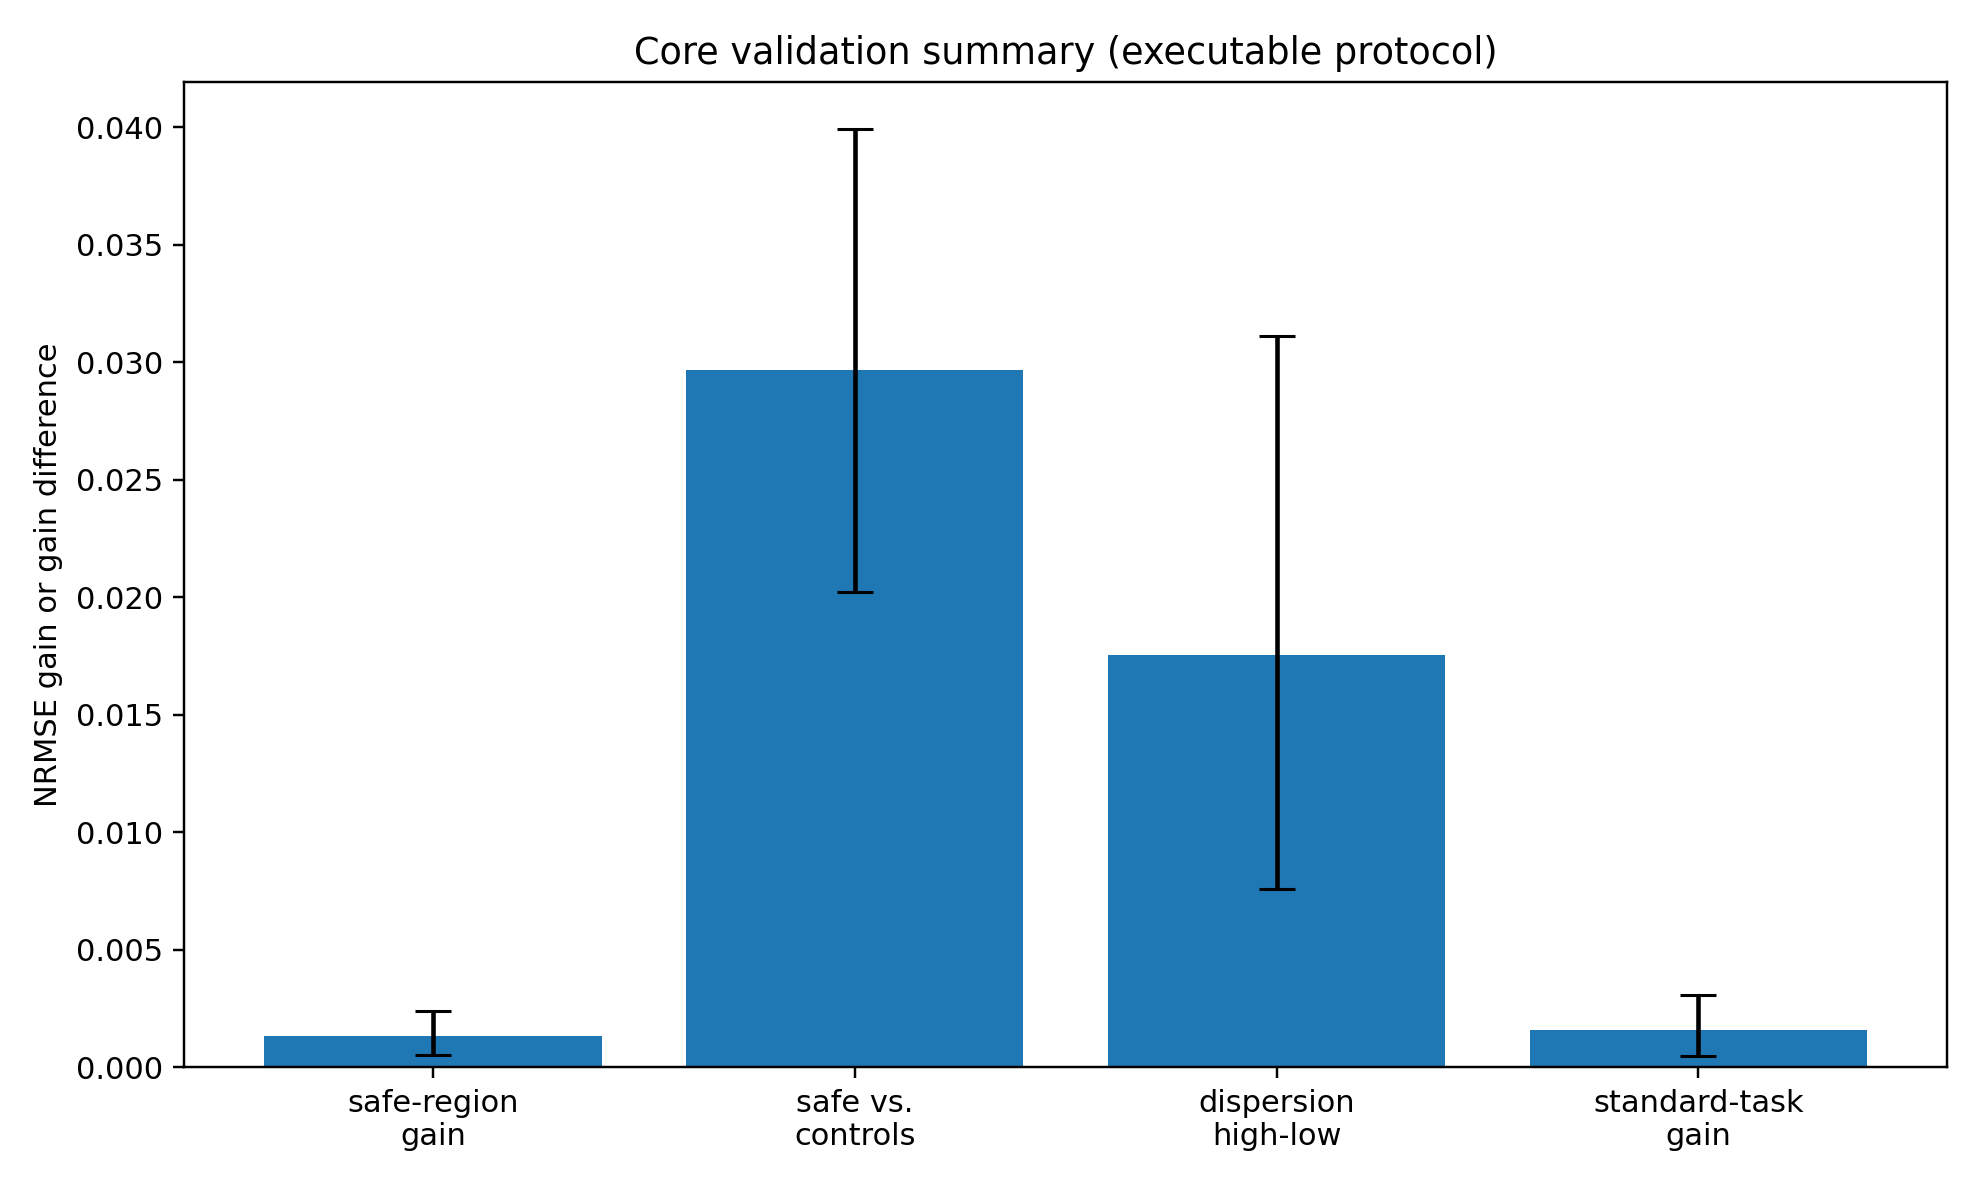
\includegraphics[width=\textwidth]{fig2_core_validation_summary.png}
\caption{Gain available inside the validation-safe region.}
\end{subfigure}
\hfill
\begin{subfigure}{0.48\textwidth}

\includegraphics[width=\textwidth]{fig3_safe_region_controls.png}
\caption{Containment compared with same-width controls.}
\end{subfigure}
\caption{Core transfer and matched-control results. Panel (a) shows the improvement available inside the validation-safe region. Panel (b) compares the validation-selected region with same-width control intervals. The two experiments use independently generated run panels, so their containment percentages are not paired estimates.}
\label{fig:m19_validation}
\end{figure}

\subsection{Do prediction differences identify windows with more available improvement?}

The path-sensitivity indicators are useful only if they are related to the improvement that target labels reveal retrospectively. Figure~\ref{fig:indicator_reliability} reports this relationship. The simplest expectation is that, when all safe temperatures produce almost identical predictions, little can be gained by choosing among them. When their predictions differ more strongly, there is more room for temperature choice to affect the result.

This expectation is supported, although the relationships are moderate rather than deterministic. Across test windows, prediction dispersion was positively correlated with the improvement available from choosing the best safe temperature ($r=0.323$). The low/high endpoint spread showed a somewhat stronger correlation ($r=0.387$). Test windows in the highest quartile of prediction dispersion had, on average, $0.01754$ more available gain than windows in the lowest quartile, with cluster-bootstrap confidence interval $[0.00760,0.03111]$. The corresponding difference for low/high endpoint spread was $0.02063$, with confidence interval $[0.00851,0.03370]$.

These results show that stronger disagreement among safe temperatures tends to occur on windows where temperature choice matters more. The relationship is moderate rather than deterministic, so the indicators are used to quantify sensitivity rather than to select a direction automatically.

\begin{figure}[t]
\centering
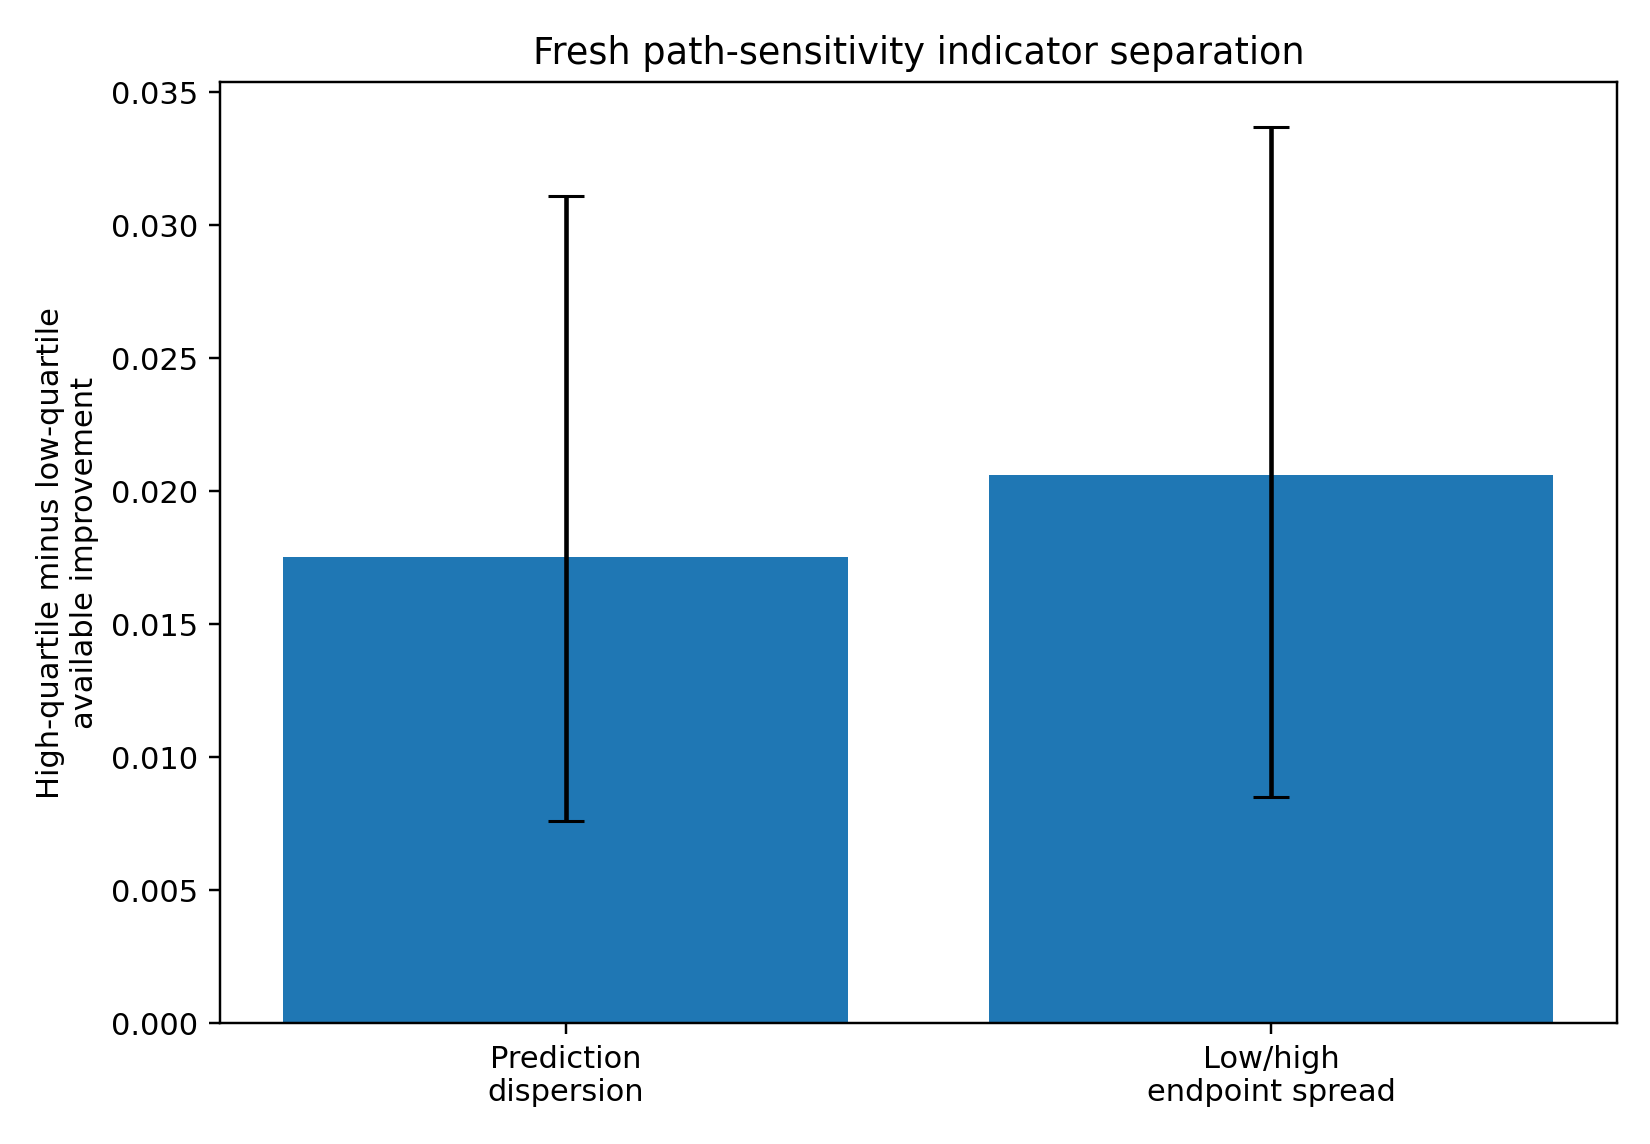
\includegraphics[width=0.62\textwidth]{fig4_path_sensitivity.png}
\caption{Windows with high prediction dispersion or high low/high endpoint spread have more available safe-region improvement than low-indicator windows. Bars show the high-quartile minus low-quartile difference in available improvement, with 95\% bootstrap confidence intervals.}
\label{fig:indicator_reliability}
\end{figure}

\subsection{When is the temperature path informative?}

The standard-task study tests how the same calibration behaves across Lorenz-$x$, Mackey--Glass, delayed memory, and NARMA10. Figure~\ref{fig:standard_boundary} shows the task-level pattern. Across the panel, the safe region contained a near-optimal test temperature in $84.4\%$ of runs and the exact best temperature on the tested grid in $68.8\%$. Mean safe-region gain was positive and averaged $0.001585$, with confidence interval $[0.000472,0.003062]$. This corresponds to about $0.16\%$ of one target standard deviation in RMSE.

The task-level differences are quantitative rather than a sharp plateau-versus-sensitive split. Mean best-safe gains range from $0.00092$ on Lorenz-$x$ to $0.00225$ on NARMA10. Full-grid gains are about $0.0055$--$0.0060$ on Lorenz-$x$, Mackey--Glass, and delayed memory, and $0.01174$ on NARMA10. Thus all four tasks leave some temperature-path opportunity, but NARMA10 exposes the clearest larger full-grid headroom in this executable panel. The path-sensitivity indicators are most informative when this headroom produces measurable prediction variation.

\begin{figure}[t]
\centering
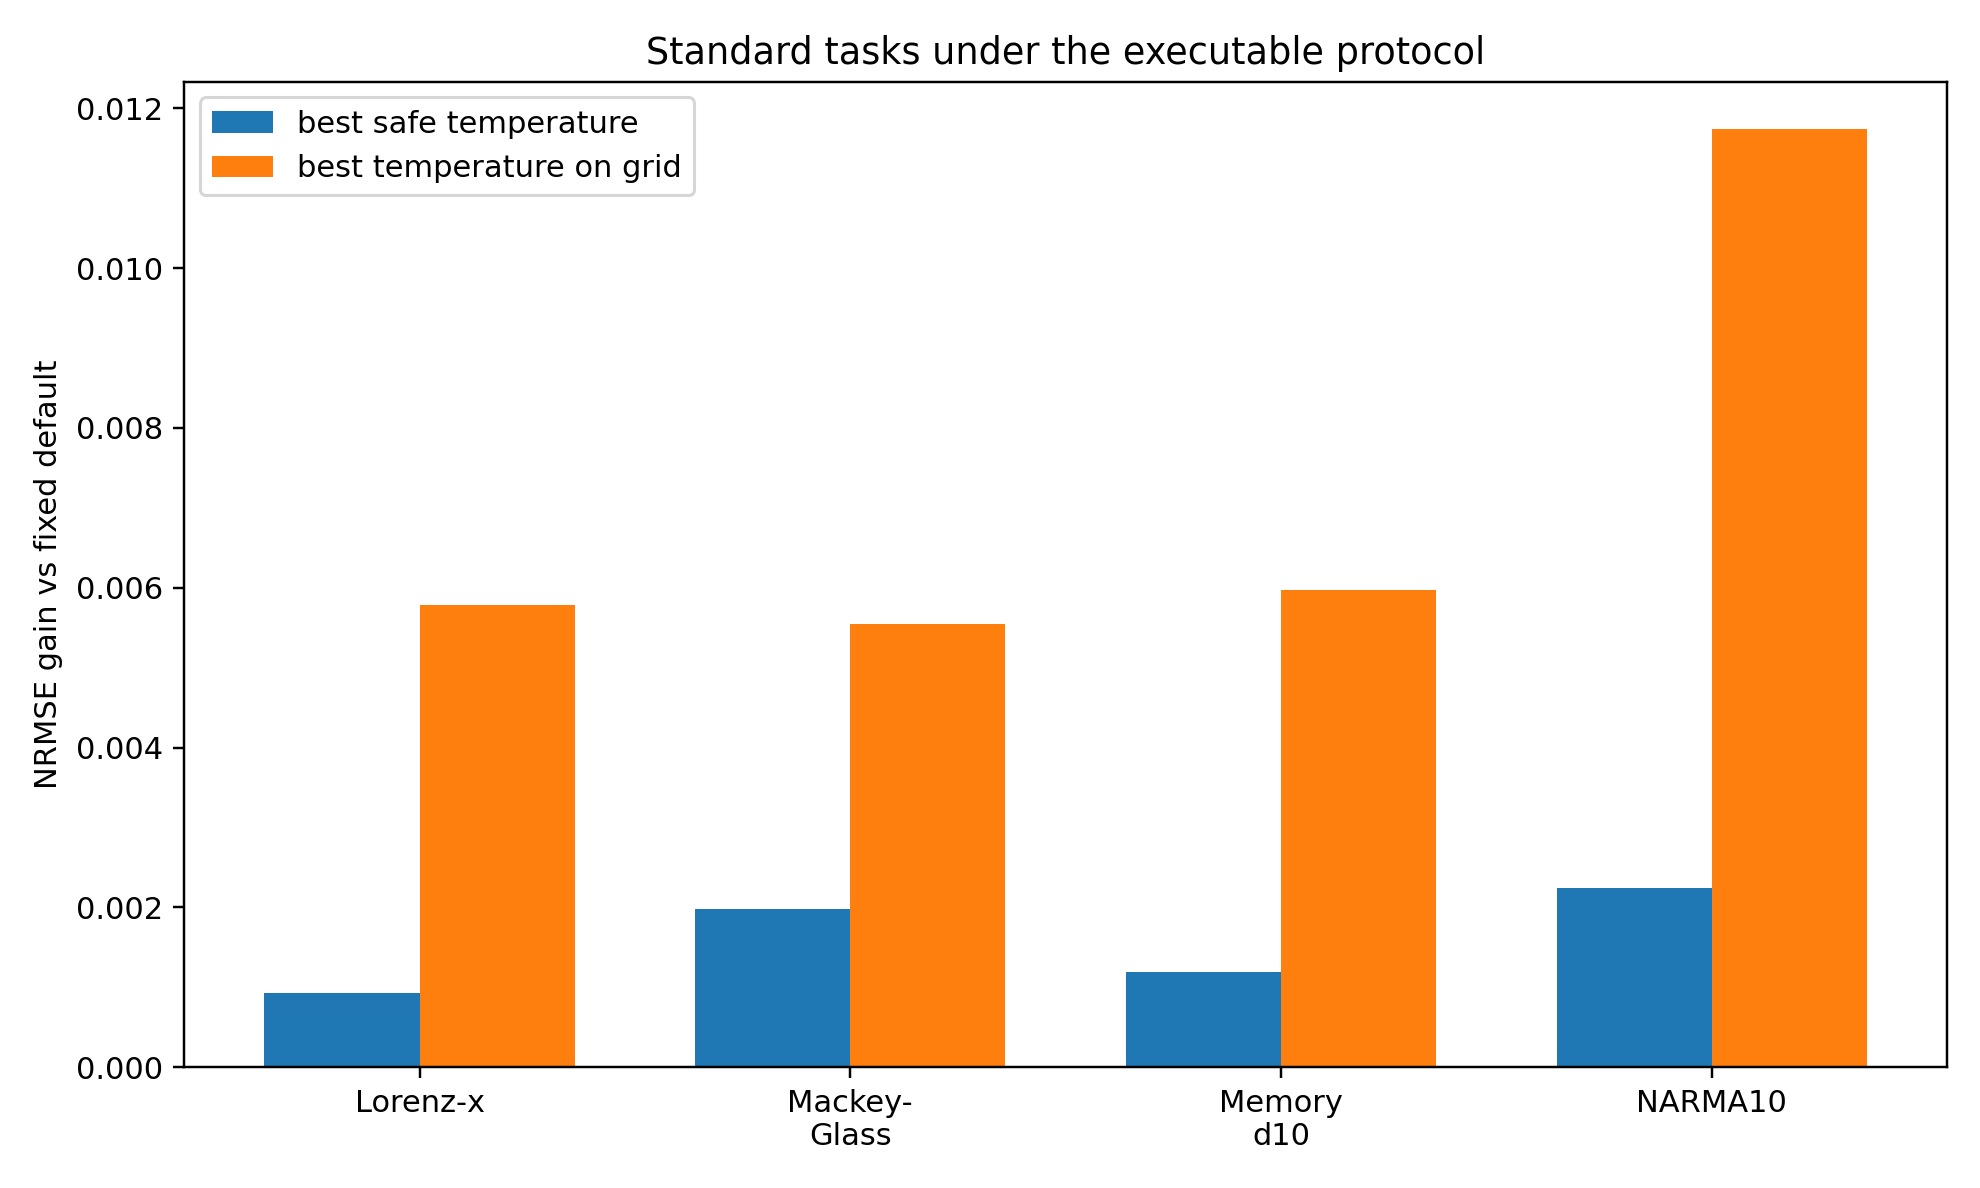
\includegraphics[width=0.70\textwidth]{fig5_standard_task_boundary.png}
\caption{The value of allocation-temperature movement depends on the task. Best-safe gains are modest on all four standard tasks, while NARMA10 shows the largest full-grid headroom in the executable panel.}
\label{fig:standard_boundary}
\end{figure}

\section{Comparison with Gain, Leak Rate, and Hard Sparsity}
\label{sec:path_ablation}

A key question is whether allocation temperature adds a genuinely different reservoir configuration axis or simply reproduces the effect of an established hyperparameter. Table~\ref{tab:path_ablation} and Fig.~\ref{fig:path_ablation} compare allocation temperature with recurrent gain, leak rate, and explicit top-$k$ sparsity under the same calibration procedure.

\begin{table}[t]
\centering
\caption{Comparison of four one-dimensional reservoir controls. Allocation temperature changes the continuous concentration of recurrent weight mass while the bulk scale is normalized. Gain changes recurrent scale, leak rate changes the update timescale, and top-$k$ sparsity changes the hard connectivity pattern.}
\label{tab:path_ablation}
\resizebox{\textwidth}{!}{%
\begin{tabular}{llllll}
\toprule
Path & Effective-support range & Spectral-radius range & Mean best-safe gain & Safe-control gain & Interpretation \\
\midrule
Temperature & $55.16$ & $0.172$ & $0.00253$ & $+0.02751$ & continuous concentration path \\
Gain & $0.00$ & $1.570$ & $0.00424$ & $+0.03453$ & amplification/spectral-radius path \\
Leak-rate & $0.00$ & $0.000$ & $0.00424$ & $+0.06149$ & update-timescale path \\
Sparsity & $58.00$ & $0.152$ & $0.00197$ & $+0.03847$ & hard top-$k$ support path \\
\bottomrule
\end{tabular}}
\end{table}

The comparison supports three conclusions. First, allocation temperature changes the concentration of recurrent weight mass in a way that gain and leak rate do not. Its mean effective-support range is $55.16$ equivalent inputs, while gain and leak-rate paths leave this concentration measure essentially unchanged. At the same time, the spectral-radius range along the temperature path is $0.172$, whereas the gain path changes spectral radius by $1.570$ while leaving effective support fixed. These complementary signatures distinguish allocation temperature from ordinary amplification. Second, the temperature safe region remains enriched relative to same-width controls: its mean safe-minus-control gain is $+0.02751$, with bootstrap interval $[0.01880,0.03679]$. Third, under the common best-safe metric, gain and leak rate provide larger within-safe-region improvement in the synthetic comparison. Allocation temperature should therefore be treated as an additional structural coordinate, not as a replacement for existing controls.

Hard sparsity is the closest structural comparison because it also changes how many inputs matter. The difference is that top-$k$ sparsity sets excluded edges exactly to zero, whereas allocation temperature continuously redistributes weight mass across the allowed edges. In this sense, allocation temperature provides a continuous concentration control that can move between highly focused and diffuse recurrent rows without changing the hard connectivity pattern. The hard-sparsity path has a similar effective-support range ($58.00$) but smaller mean best-safe improvement ($0.00197$) than allocation temperature ($0.00253$) in this comparison.

\begin{figure}[t]
\centering
\begin{subfigure}{0.48\textwidth}
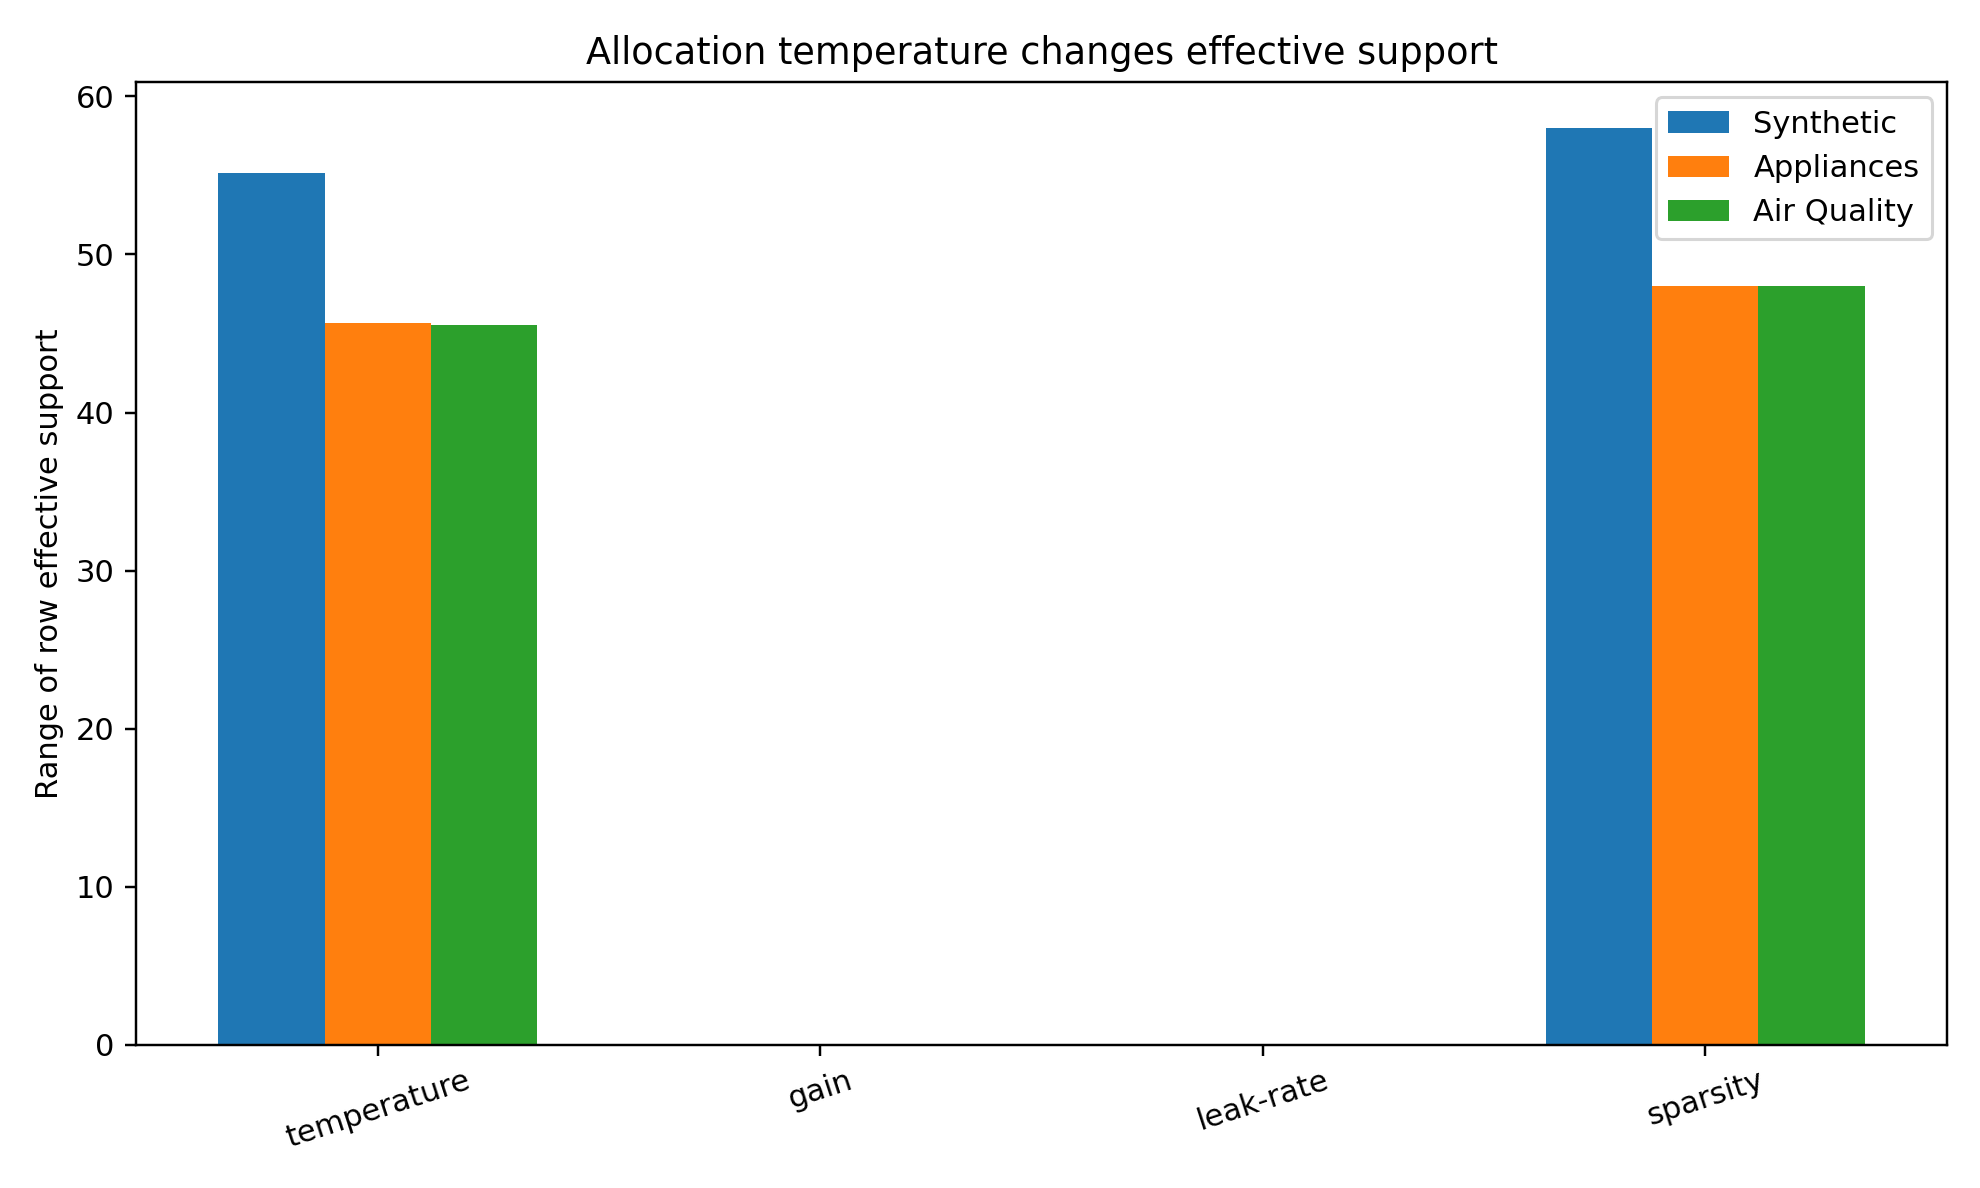
\includegraphics[width=\textwidth]{fig6_structural_ablation.png}
\caption{Support range by path.}
\end{subfigure}
\hfill
\begin{subfigure}{0.48\textwidth}
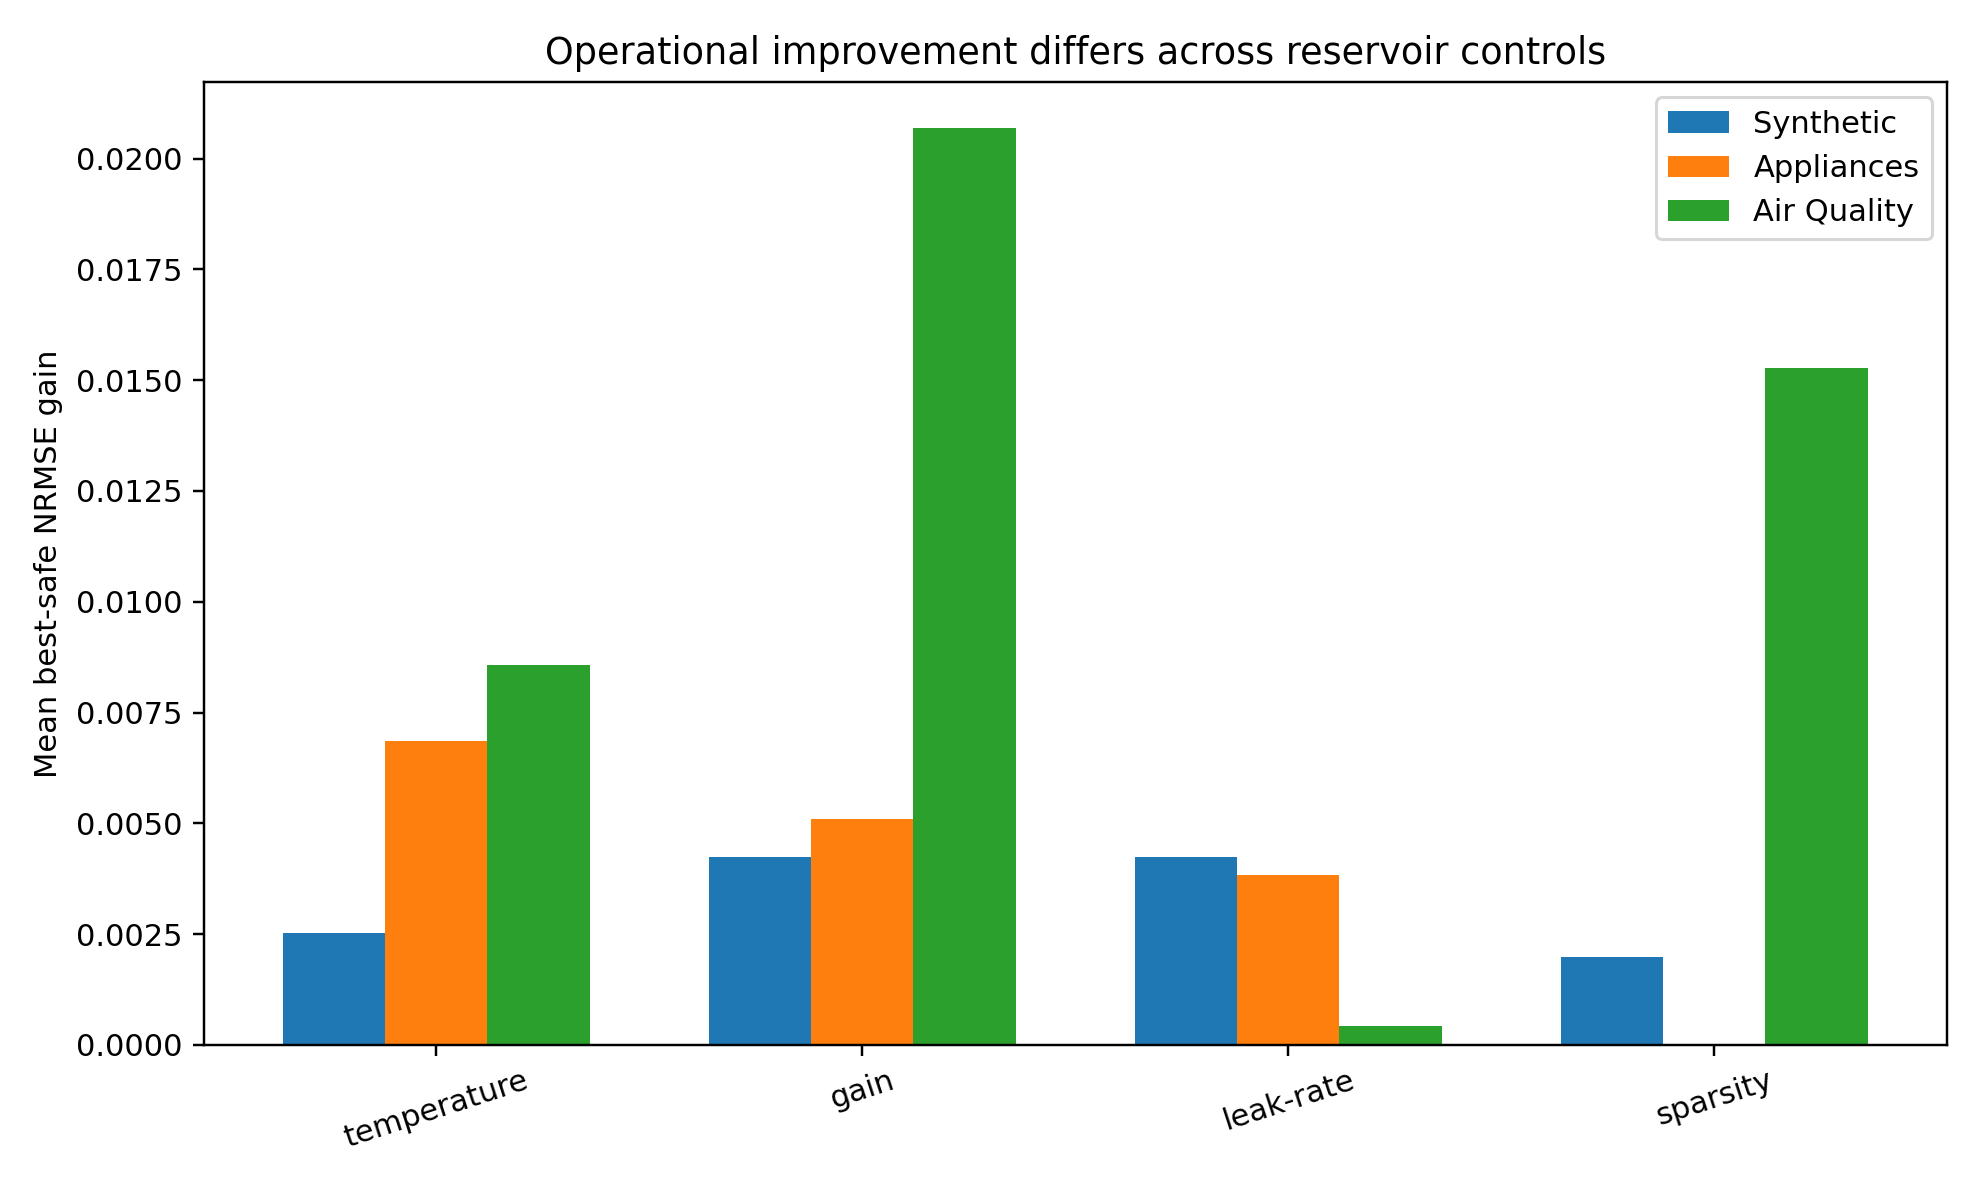
\includegraphics[width=\textwidth]{fig7_operational_ablation.png}
\caption{Improvement available inside each validation-safe region.}
\end{subfigure}
\caption{Path ablations. Allocation temperature and sparsity change recurrent support; gain and leak-rate do not. Panel (b) reports mean best-safe NRMSE gain under a common metric across controls and across the synthetic and two real-data panels. Operationally, allocation temperature is useful and structurally distinct but not dominant over all one-dimensional paths.}
\label{fig:path_ablation}
\end{figure}

\section{Real-World Sensor Benchmarks}
\label{sec:real_world}

Table~\ref{tab:real_world} applies the same calibration procedure to two public sensor time-series datasets. The first study uses the UCI Appliances Energy Prediction dataset \citep{candanedo2017accurate}. The task predicts $\log(1+\mathrm{Appliances}_{t+h})$ from current appliance use, indoor sensor variables, weather variables, and time encodings, with horizon $h=6$ samples, approximately one hour in the original ten-minute sampling. The second study uses the UCI Air Quality dataset \citep{devito2008field}. The task predicts future benzene concentration $\mathrm{C6H6(GT)}$ from current multivariate chemical-sensor and meteorological measurements, with horizon one hour.

\begin{table}[t]
\centering
\caption{Executable four-split real-world sensor benchmark summary. Appliances Energy yields a null safe-region-versus-control result, whereas Air Quality gives a positive result. Path indicators report the correlation of prediction dispersion and low/high endpoint spread with available best-safe improvement.}
\label{tab:real_world}
\resizebox{\textwidth}{!}{%
\begin{tabular}{lllllll}
\toprule
Dataset & Rows/features & Target & Temp. support range & Temp. mean best-safe gain & Temp. safe $-$ control & Temp. path indicators \\
\midrule
Appliances Energy & $19729/32$ & log future appliances, $h=6$ & $45.69$ & $0.00685$ & $-0.00935$ [$-0.03275$, $0.01933$] & $0.673$ / $0.640$ \\
Air Quality & $9356/19$ & future C6H6, $h=1$ & $45.52$ & $0.00856$ & $+0.03925$ [$0.01110$, $0.07962$] & $0.489$ / $0.459$ \\
\bottomrule
\end{tabular}}
\end{table}

The four-split executable panel provides complementary evidence for how the allocation-temperature axis behaves on measured sensor data. On Appliances Energy, allocation temperature retains its structural signature and both path-sensitivity indicators are positively associated with available improvement, but the mean safe-region-minus-control gain is negative ($-0.00935$) and its confidence interval crosses zero ($[-0.03275,0.01933]$). This is a null result for safe-region localization on that dataset. The mean best-safe temperature gain itself is positive ($0.00685$), but the validation-selected interval is not more informative than same-width alternatives.

On Air Quality, the temperature safe region gives a positive safe-minus-control result of $+0.03925$ with confidence interval $[0.01110,0.07962]$. Prediction dispersion and low/high endpoint spread remain positively correlated with the improvement available inside the safe region ($r=0.489$ and $0.459$). The mean best-safe temperature gain is $0.00856$. Temperature is not the strongest operational path on this dataset in the regenerated panel: gain and hard sparsity provide larger mean best-safe gains. The real-data conclusion is therefore deliberately mixed: allocation temperature transfers as a distinct structural coordinate and can support useful validation localization, but that localization is dataset-dependent and does not imply operational dominance over established controls.



\section{Additional Validation of Sensitivity and Structural Confounds}
\label{sec:additional_validation}

This section tests whether the main conclusions depend on the width of the validation-safe region, the tolerance used to define it, or unintended changes in spectral radius. It also separates the continuous path-sensitivity result from a less stable binary threshold summary.

\subsection{Safe-region width and tolerance sensitivity}

The validation safe region is intentionally conservative. At the default relative tolerance $\epsilon_{\mathrm{rel}}=0.10$, using each study's native absolute floor, the mean temperature-safe widths are $2.89$ candidate points in the synthetic path-comparison study and $2.75$ candidate points in each real-data study (Table~\ref{tab:m21_safe_width}). Relative to all same-width intervals on the same grid, near-optimal containment is enriched by $2.36\times$ in the synthetic comparison and $1.39\times$ on Air Quality. Appliances Energy is the important counterexample: its ratio is $0.69\times$, consistent with the null safe-minus-control result above. These finite-grid quantities show that validation localization can be informative but is not guaranteed to be so on every dataset.

For the executable synthetic M20a audit, sensitivity checks over $\epsilon_{\mathrm{rel}}\in\{0.05,0.10,0.15,0.20\}$ preserve the qualitative conclusion. Mean safe width increases from $2.50$ to $3.43$ candidates, while near-optimal containment remains $85.7\%$ and the containment ratio relative to same-width controls remains above one, decreasing from $2.79\times$ to $1.87\times$ as the accepted region widens. The mean safe-minus-control gain remains positive throughout ($0.03078$ to $0.02426$).

\begin{table}[t]
\centering
\caption{Safe-region width at $\epsilon_{\mathrm{rel}}=0.10$ using each study's native absolute tolerance. The controlled synthetic panel and Air Quality show containment enrichment over same-width controls, while Appliances Energy provides a null/counterexample. Mean best-safe gain uses the same definition in all rows.}
\label{tab:m21_safe_width}
\resizebox{\textwidth}{!}{%
\begin{tabular}{llllll}
\toprule
Study & $\epsilon_{\mathrm{abs}}$ & Mean safe width & Width fraction & Near-optimal containment ratio & Mean best-safe gain \\
\midrule
Synthetic path comparison & $0.005$ & $2.89/13$ & $22.3\%$ & $2.36\times$ & $0.00253$ \\
Appliances Energy & $0.002$ & $2.75/13$ & $21.2\%$ & $0.69\times$ & $0.00685$ \\
Air Quality & $0.002$ & $2.75/13$ & $21.2\%$ & $1.39\times$ & $0.00856$ \\
\bottomrule
\end{tabular}}
\end{table}

\subsection{Reliability of the path-sensitivity indicators}

The main result is continuous: windows with greater prediction dispersion or greater low/high endpoint spread tend to have more improvement available from choosing among the safe temperatures. A secondary analysis converted each indicator into a top-quartile binary flag and asked whether flagged windows were more likely to have positive gain. That threshold result is less stable when grid density or reservoir size changes. We therefore retain the continuous association as the primary result and report the binary threshold tables separately in Appendix~\ref{app:binary_threshold}.

\subsection{Separating allocation temperature from gain and hard sparsity}

The structural audit separates support from gain. Tables~\ref{tab:path_ablation} and \ref{tab:real_world} show that allocation temperature changes effective support substantially, whereas gain and leak-rate leave it approximately fixed. The complementary spectral-radius comparison points in the opposite direction. Gain changes spectral radius by about $1.47$--$1.61$ in the synthetic comparison and the two real-data studies, while allocation temperature changes it much less ($0.172$, $0.175$, and $0.152$). The two controls therefore affect different measurable properties: gain primarily changes recurrent amplification, whereas allocation temperature primarily changes the concentration of recurrent weight mass.

Hard sparsity is the closest structural comparator because it also changes how recurrent influence is distributed across inputs. The distinction is both structural and operational. Sparsity imposes hard top-$k$ truncation, setting excluded edges to zero. Allocation temperature continuously redistributes recurrent weight mass over the same candidate row, preserving graded weights. In the path comparison, sparsity has support range $58.00$ and mean best-safe gain $0.00197$, whereas the allocation-temperature path has comparable support expansion and mean best-safe gain $0.00253$ (Table~\ref{tab:path_ablation}). On Air Quality, gain and hard sparsity provide larger mean best-safe gains than temperature, reinforcing the conclusion that structural distinctness does not imply operational dominance. Allocation temperature therefore provides a continuous concentration control that is distinct from hard support selection.


\section{Robustness to Grid Density and Reservoir Size}
\label{sec:grid_size_robustness}

This robustness study changes one experimental factor at a time. It retains delayed memory, NARMA10, and Lorenz-$x$, and adds a controlled delayed-signal task with a non-predictive distractor channel. The controlled task has a known delayed target relationship, which makes it useful for checking whether the conclusions survive changes in temperature-grid density and reservoir size. Each task is evaluated over four trials with train/validation/test lengths $1200/500/500$ and a 100-step washout. The baseline configuration is $N=60,K=13$. A nested $K=25$ temperature grid changes only the grid density at $N=60$ while reusing the same data and reservoir substrate. The $N=150,K=13$ configuration changes only reservoir size. For each configuration, the validation-safe region and all same-width control intervals are recomputed from that configuration's validation results. Table~\ref{tab:m23_robustness} summarizes the containment and indicator results, and Table~\ref{tab:m23_absolute_performance} gives the absolute NRMSE values.

A safe region containing a single temperature still contributes to the containment and gain analyses. The two path-sensitivity indicators, however, quantify variation across multiple candidate predictions, so they require at least two distinct safe temperatures. Singleton cases are therefore omitted from the indicator-correlation analysis. The primary robustness question is whether the continuous relationship between prediction variation and available safe-region improvement persists. A separate binary top-quartile analysis is retained only as a secondary summary.

\begin{table}[t]
\centering
\caption{Grid-density and reservoir-size robustness. Indicator correlations measure the relationship between test-window prediction variation and the improvement available from choosing the best temperature inside the validation-safe region. The secondary binary threshold analysis is reported in Appendix~\ref{app:binary_threshold}.}
\label{tab:m23_robustness}
\resizebox{\textwidth}{!}{%
\begin{tabular}{lllllll}
\toprule
Configuration & Safe width & Near-optimal containment ratio & Best-point containment ratio & Safe $-$ control gain & Disp. corr. & Endpoint corr. \\
\midrule
$N=60,K=13$ & $20.7\%$ & $2.864\times$ & $3.513\times$ & $+0.03397$ & $0.452$ & $0.410$ \\
$N=60,K=25$ & $17.5\%$ & $2.160\times$ & $5.014\times$ & $+0.02725$ & $0.515$ & $0.513$ \\
$N=150,K=13$ & $18.8\%$ & $2.257\times$ & $3.304\times$ & $+0.02043$ & $0.577$ & $0.566$ \\
\bottomrule
\end{tabular}}
\end{table}

\begin{table}[t]
\centering
\caption{Absolute test-performance context for the reference robustness configuration ($N=60,K=13$), averaged over four fixed trials per task. Safe reduction is $(\mathrm{NRMSE}_{\mathrm{default}}-\mathrm{NRMSE}_{\mathrm{best\ safe}})/\mathrm{NRMSE}_{\mathrm{default}}$. The best-grid value is computed retrospectively and shows the remaining improvement available over the tested temperature grid.}
\label{tab:m23_absolute_performance}
\resizebox{\textwidth}{!}{%
\begin{tabular}{lllll}
\toprule
Task & Default test NRMSE & Best-safe test NRMSE & Best-grid NRMSE & Safe reduction \\
\midrule
Controlled delayed signal & $0.92665$ & $0.91713$ & $0.90874$ & $1.03\%$ \\
Delayed memory & $0.77276$ & $0.77136$ & $0.77069$ & $0.18\%$ \\
NARMA10 & $0.66285$ & $0.65836$ & $0.65836$ & $0.68\%$ \\
Lorenz-$x$ & $0.03269$ & $0.03206$ & $0.02254$ & $1.91\%$ \\
\bottomrule
\end{tabular}}
\end{table}

Table~\ref{tab:m23_absolute_performance} makes the practical magnitude explicit. In the baseline robustness setting, selecting the best temperature inside the validation-safe component reduces default test NRMSE by $0.18\%$--$1.91\%$ across tasks. These are modest NRMSE reductions obtained by choosing among temperatures that validation had already accepted. The best candidate over the full tested grid is reported separately as a retrospective reference. The core robustness conclusion is stable. Mean safe-region width remains between $17.5\%$ and $20.7\%$ of the candidate grid. Near-optimal containment occurs more than twice as often in the validation-safe region as in same-width control intervals, and exact-best containment occurs more than three times as often. These ratios describe enrichment in containment frequency. The corresponding prediction-error changes are reported separately in Table~\ref{tab:m23_absolute_performance}. Temperature also continues to sweep a large structural range: the effective-support range is $0.919N$, $0.919N$, and $0.943N$ in the three configurations, where $N$ is the number of reservoir units, while spectral-radius ranges remain $0.182$, $0.189$, and $0.138$, respectively. Thus the safe-region enrichment persists beyond the original $K=13,N=60$ setting, while the numerical containment ratios remain empirical quantities for the tested grids and reservoirs.

The path-sensitivity result is more nuanced. Safe-region dispersion and anchor spread remain positively correlated with available safe-region improvement in every configuration, with correlations between $0.410$ and $0.577$. High-minus-low mean available improvement has a positive point estimate for both primary indicators in all configurations. For $N=150$, however, only 11 of 16 cases have multi-point safe regions and the bootstrap interval includes zero; the larger-reservoir result is therefore directionally consistent with the smaller configurations but does not independently confirm a nonzero high-versus-low difference. The binary top-quartile statistic behaves differently. Its precision ratio is close to one in the baseline configuration and below one after increasing grid density or reservoir size, with intervals crossing one. The stable result is therefore the continuous association: larger prediction variation along the calibrated temperature path tends to accompany more available improvement. The usefulness of a fixed binary threshold depends on the tested grid, reservoir size, and base rate of positive gain.

\begin{figure}[t]
\centering
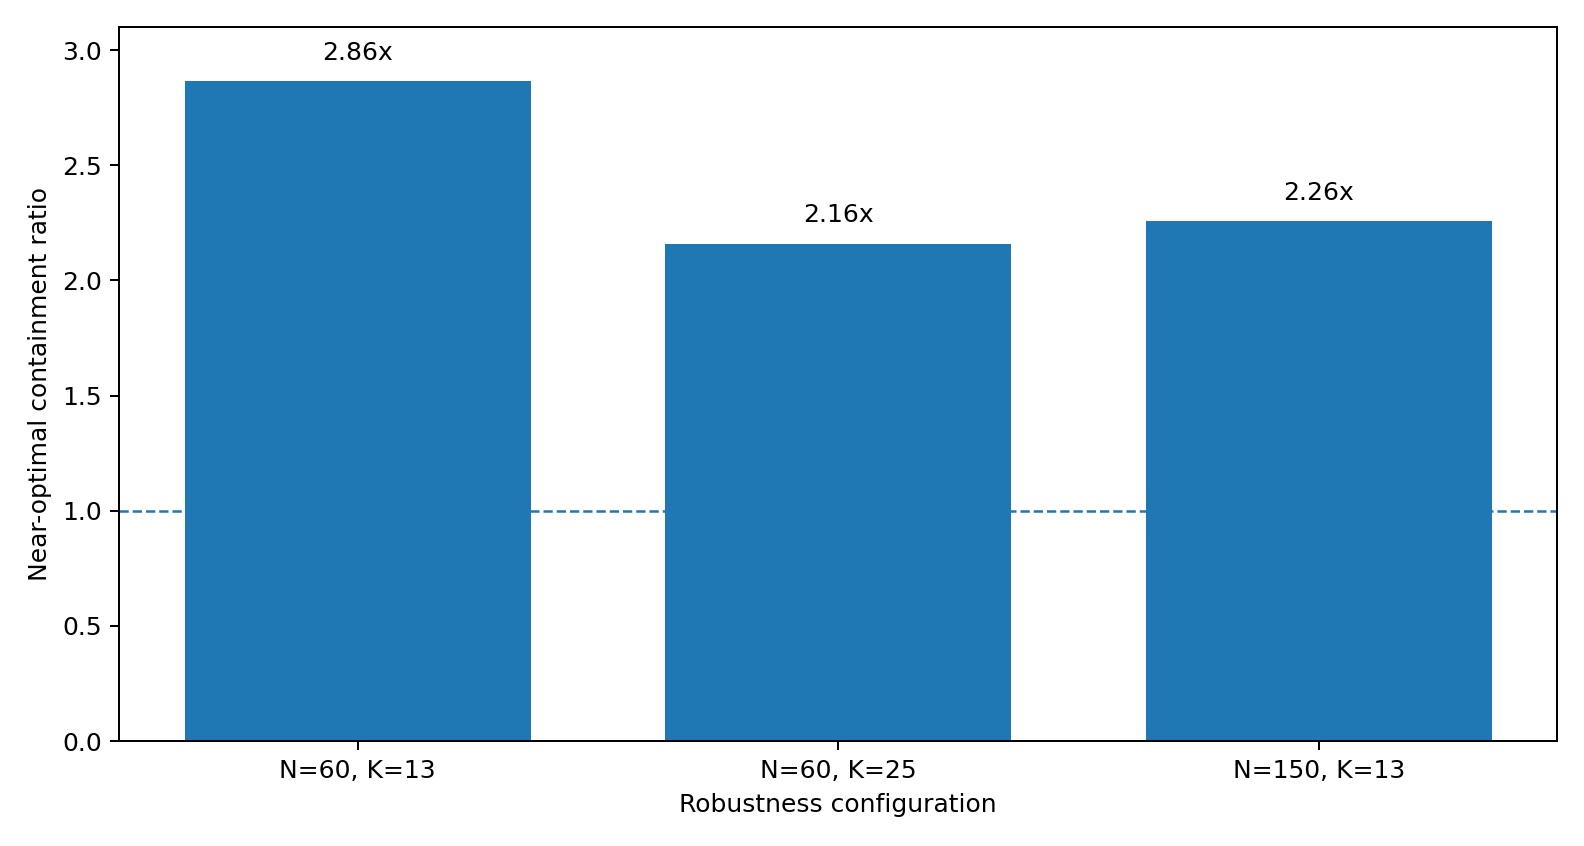
\includegraphics[width=0.78\textwidth]{fig8_robustness_containment.png}
\caption{Near-optimal containment relative to same-width control intervals under the three robustness configurations. The validation-safe region remains enriched after increasing temperature-grid density or reservoir size. Continuous indicator correlations for the same configurations are reported in Table~\ref{tab:m23_robustness}.}
\label{fig:m23_robustness}
\end{figure}

\section{Structural Opportunity Under Distribution Shift}
\label{sec:shift_audit_results}

This is the final validation section. The earlier experiments ask how much can be gained by choosing among temperatures that remain inside a one-dimensional validation-safe region. Here the candidate set is deliberately broader: an $11\times11$ temperature--leak grid. The aim is to measure how much improvement is available under distribution shift when a second structural control is added, and then to test how much of that improvement can be recovered without target labels. The one-dimensional path indicators and this two-dimensional study therefore answer complementary questions. The former measure sensitivity inside an already accepted temperature region; the latter measures the larger structural opportunity and the difficulty of identifying low-error structures from unlabeled target data.

\subsection{Upper-bound benefit of target-specific structural combinations}

Table~\ref{tab:shift_task_results} compares three quantities on the full 121-candidate set. The fixed baseline is the single structure chosen from the pre-deployment conditions. The pre-deployment sparse ensemble can combine up to five structures, but its weights are also fixed before held-out evaluation. The third quantity is an upper bound: a five-model ensemble fitted retrospectively with the target values from each held-out window.

\begin{table}[H]
\centering
\caption{Distribution-shift results by task. NRMSE values are averaged over held-out shift types and three independent reservoir substrates. Relative gains use $(L_{\mathrm{fixed}}-L_{\mathrm{policy}})/L_{\mathrm{fixed}}$. Because only three substrates are available per task, the main table reports the observed task means rather than emphasizing resampled task-specific confidence intervals.}
\label{tab:shift_task_results}
\small
\setlength{\tabcolsep}{4.5pt}
\resizebox{\textwidth}{!}{%
\begin{tabular}{lccccc}
\toprule
Task & Fixed & \shortstack{Pre-deployment\\ensemble} & \shortstack{Target-label\\upper bound} & \shortstack{Ensemble\\gain} & \shortstack{Upper-bound\\gain} \\
\midrule
NARMA10 & 1.0064 & 0.8854 & 0.7518 & 12.02\% & 25.30\% \\
Mackey--Glass & 0.6193 & 0.4959 & 0.3776 & 19.93\% & 39.03\% \\
Lorenz-$x$ & 0.6577 & 0.5274 & 0.4367 & 19.82\% & 33.60\% \\
\bottomrule
\end{tabular}}
\end{table}

The target-label upper bound reduces NRMSE by $25.3\%$--$39.0\%$ relative to the fixed structure selected before deployment. Because each task contains only three independent reservoir substrates, the task means and their consistency across tasks carry the claim. We therefore do not emphasize task-specific resampled intervals in the main table. These reductions are much larger than the improvements available inside the one-dimensional validation-safe temperature region. The experiments are intentionally different: the upper bound can combine structures from a 121-candidate temperature--leak bank and uses target labels from each held-out window. It therefore measures the amount of structural improvement available in principle under shift.

The sparse ensemble fitted only on pre-deployment conditions reduces task-level NRMSE by $12.0\%$--$19.9\%$. Relative to the target-label upper bound, it recovers approximately $48\%$--$59\%$ of the available reduction. A fixed combination of complementary structures can therefore recover a meaningful part of the shift-specific opportunity without held-out target labels, while a substantial gap remains.

\subsection{Predicting low-error structures without target labels}

The unlabeled error-prediction model does not close that gap. Its mean NRMSE is 0.9135 on NARMA10, 0.5403 on Mackey--Glass, and 0.5422 on Lorenz-$x$, compared with 0.8854, 0.4959, and 0.5274 for pre-deployment sparse ensemble. It improves on the fixed baseline at the task-average level, but is worse than the simpler pre-deployment sparse ensemble on all three tasks.

The error-prediction model uses structural coordinates, clean-validation and pre-deployment error, predictive disagreement and variance, perturbation consistency, and reservoir-state shift diagnostics. Even with these features, it does not transfer reliably enough to rank the candidate structures by held-out target error. This result reinforces the distinction developed earlier: prediction variation can reveal structural sensitivity, while estimating which structure will be most accurate is harder without target labels.

\subsection{Performance across shift types and cost of pre-deployment certification}

The average benefit of the pre-deployment sparse ensemble depends strongly on the type of held-out shift (Table~\ref{tab:shift_family_results}). It is positive under stronger correlated additive noise and offset drift, but reverses under block missingness.

\begin{table}[H]
\centering
\caption{Pre-deployment sparse ensemble by held-out shift type. Relative gains are computed against the pre-deployment fixed structure. Intervals resample the nine task--substrate clusters and retain all windows within each cluster. They remain finite-panel descriptive summaries. A negative gain denotes degradation.}
\label{tab:shift_family_results}
\scriptsize
\setlength{\tabcolsep}{4pt}
\begin{tabular}{>{\raggedright\arraybackslash}p{0.30\textwidth}cccc}
\toprule
Held-out shift & \shortstack{Pre-deployment\\fixed} & \shortstack{Sparse\\ensemble} & \shortstack{Relative gain\\{[95\% CI]}} & \shortstack{Windows\\harmed} \\
\midrule
Strong correlated additive noise & 1.4606 & 0.9771 & 33.10\% [23.08, 41.61] & 0/36 \\
Offset drift & 0.6950 & 0.5932 & 14.65\% [11.18, 16.82] & 16/72 \\
Block missingness & 0.4776 & 0.5088 & $-6.55\%$ [$-15.11$, $-0.49$] & 45/72 \\
\bottomrule
\end{tabular}
\end{table}

Under block missingness, aggregation harms 45 of 72 held-out windows (62.5\%), and the cluster-bootstrap interval remains below zero. The pre-deployment sparse ensemble is therefore beneficial on average across the task panel, but its reliability depends on the type of shift. The failure is especially important because block missingness removes information rather than only perturbing its scale or adding noise; a fixed combination of structural experts cannot restore observations that are absent.

Restricting the set of structures available to the target-label upper bound also has a measurable cost. We define the aggregate relative price of certification as
\begin{equation}
  C_{\mathrm{cert}}
  =\frac{L^{\star}_{\mathrm{cert}}-L^{\star}_{\mathrm{global}}}
  {L^{\star}_{\mathrm{global}}},
  \label{eq:certification_cost}
\end{equation}
Here $L^{\star}_{\mathrm{global}}$ is the mean NRMSE of the target-label upper-bound ensemble when it can choose from all 121 structures. $L^{\star}_{\mathrm{cert}}$ is the corresponding mean when the ensemble is restricted to the pre-deployment certified subset. Both use the same five-model nonnegative ensemble class. The cost is 4.98\% for Lorenz-$x$ (descriptive 95\% interval 3.02--8.93\%), 9.61\% for Mackey--Glass (7.05--14.37\%), and 8.29\% for NARMA10 (1.86--16.76\%). The certified subset therefore reduces the number of structures that can be considered at deployment, but it also excludes some combinations that perform well on particular held-out shifts. The percentages above quantify that performance trade-off.

\section{Discussion}
\label{sec:discussion}

The main contribution is a new structural configuration axis for reservoir computing. Allocation temperature continuously controls how recurrent weight mass is concentrated across each row while recurrent scale is normalized separately. This provides a continuous control of recurrent weight concentration without changing the hard connectivity pattern, and a configuration dimension that is empirically distinct from gain and leak rate. The analytical characterization establishes monotonic control of allocation entropy and effective support. The experiments then characterize this axis under validation, on measured sensor data, under changes in grid density and reservoir size, and under distribution shift.

The controlled one-dimensional safe-region experiments show two complementary properties. First, validation selects temperature intervals that contain near-optimal test points more often than same-width control intervals. Second, test-window prediction variation across those accepted temperatures is positively associated with the improvement that target labels reveal retrospectively. The real-data panel then shows that the first property is not universal: Air Quality remains positively localized, whereas Appliances Energy is a null case. The direct NRMSE reduction available inside the safe region is modest in the reference robustness panel ($0.18\%$--$1.91\%$ from the validation-selected default). Their main value is diagnostic: they show when recurrent allocation choice matters on the current window. The continuous relationship persists when the temperature grid is made denser and when the reservoir grows to $N=150$. The binary top-quartile rule is less stable and is retained only as a secondary analysis in Appendix~\ref{app:binary_threshold}.

The path comparison clarifies why allocation temperature should be treated as an additional reservoir dimension rather than a renamed gain or sparsity parameter. Temperature changes continuous row concentration with relatively small spectral-radius variation. Gain strongly changes spectral radius while leaving row concentration fixed. Leak rate changes update timescale. Hard sparsity changes the zero/nonzero edge pattern. No single path dominates every task operationally, but their different structural signatures make them complementary controls.

The distribution-shift study broadens the question from sensitivity along one accepted temperature path to structural model choice over a two-dimensional temperature--leak bank. The target-label upper bound shows that substantial improvement is available when target errors are known. The pre-deployment sparse ensemble recovers roughly half of that reduction at the task-average level without using held-out labels. The unlabeled error-prediction model does not outperform that simpler ensemble, which shows that estimating target error from unlabeled target statistics remains difficult. The failure under block missingness is especially informative: a fixed structural ensemble cannot compensate for information that is absent from the input.

Operationally, low path sensitivity supports retaining the validation-selected default, whereas high sensitivity should be treated as a monitoring signal rather than an automatic direction of movement. A fuller decision-oriented interpretation is provided in Appendix~\ref{app:operational_interpretation}.



The validation-safe temperature region $\mathcal T_{\mathrm{safe}}$ and the two-dimensional certified subset $\Theta_{\mathrm{cert}}$ serve related but different purposes. The former is a connected interval around the validation-selected temperature. The latter is a pre-deployment filter over a temperature--leak grid. Restricting the target-label upper bound to $\Theta_{\mathrm{cert}}$ increases mean loss by about $5\%$--$10\%$ across the three shift-study tasks. This quantifies the trade-off between conservative pre-deployment filtering and access to structures that become useful only under particular target shifts.

The executable real-world panel is consistent with the same bounded interpretation. Appliances Energy gives a null safe-region-versus-control result even though its path-sensitivity correlations are positive. Air Quality gives a positive safe-region-versus-control result, but temperature is not the strongest one-dimensional operational path there. The structural coordinate therefore transfers to measured sensor data, while the usefulness of validation localization remains dataset-dependent.

\section{Limitations}
\label{sec:limitations}

The results define a useful but bounded scope for the method.
\begin{enumerate}[leftmargin=*]
  \item The path-sensitivity indicators do not identify the temperature with the lowest target error. Without target labels, the validation-selected default remains the justified automatic choice unless a separate fallback policy has been validated.
  \item The distribution-shift study shows that unlabeled prediction and state statistics are not sufficient, in the evaluated setting, to reliably rank all structural candidates by target error. The target-label upper bound is therefore an upper bound on available improvement rather than a deployable adaptation rule.
  \item The pre-deployment sparse ensemble is shift-dependent. It improves performance under stronger correlated noise and offset drift, but degrades under block missingness. Information-removing shifts require additional mechanisms.
  \item Allocation temperature is structurally distinct from gain, leak rate, and hard sparsity, but it does not dominate them on every task. Its main contribution is a new, interpretable structural coordinate and a calibration framework for studying that coordinate.
  \item RMS normalization controls bulk recurrent scale but does not hold spectral radius exactly constant. The relatively small spectral-radius variation along the temperature path supports its distinction from a pure gain path, but does not establish complete dynamical independence between allocation concentration and recurrent amplification.
  \item The real-data evaluation uses four chronological splits per dataset. Air Quality provides a positive safe-region-versus-control result, whereas Appliances Energy is a null case. These split-level panels support transfer beyond synthetic tasks but remain small finite-sample studies rather than broad application benchmarks.
  \item The evaluated reservoirs range from $N=45$ to $N=150$, with temperature grids of 13 or 25 points in the one-dimensional studies. Larger reservoirs, alternative raw-score distributions, sparse or modular topologies, physical reservoirs, and joint changes of grid density and reservoir size remain to be tested.
  \item Some uncertainty summaries contain few independent higher-level units. In the distribution-shift study, only three independent reservoir substrates are available per task, so Table~\ref{tab:shift_task_results} reports the observed task means without emphasizing task-specific bootstrap intervals. The shift-type intervals in Table~\ref{tab:shift_family_results} resample nine task--substrate clusters and should still be interpreted as finite-panel uncertainty summaries.
  \item The entropy result characterizes the recurrent allocation itself. It does not prove task optimality, echo-state guarantees, or universal improvements in memory capacity as temperature changes.
\end{enumerate}

\section{Conclusion}
\label{sec:conclusion}

Allocation temperature adds a distinct structural coordinate to reservoir computing by controlling how recurrent weight mass is distributed while bulk recurrent scale is normalized separately. Its row entropy and effective support increase monotonically with temperature, distinguishing it from gain, leak rate, and hard sparsity.

Validation-safe temperature regions are enriched for useful held-out operating points in the controlled panels, and prediction variation across those regions indicates when recurrent allocation matters more strongly. The effect is not universal: Air Quality shows positive localization whereas Appliances Energy is a null case, and direct within-region NRMSE gains remain modest. Robustness to a denser grid and larger reservoirs supports the structural interpretation while also showing that continuous sensitivity measures are more stable than fixed binary thresholds.

Under broader temperature--leak distribution shift, target labels reveal substantially more structural opportunity than unlabeled target statistics can reliably identify. A pre-deployment sparse ensemble recovers part of that opportunity but fails under block missingness. Allocation temperature therefore provides an interpretable reservoir-design coordinate and a controlled framework for distinguishing structural sensitivity, available improvement, and the limits of label-free adaptation.

\section*{Code and Data Availability}

The public reproducibility package is available in the \href{https://github.com/ildefons/temperature-calibrated-reservoirs}{project repository}. It contains the manuscript source, generated tables and figures, environment specifications, computational notebooks, executable result files, and verification checks. Appendix~\ref{app:repro_map} maps each main-text result to the corresponding computational artifact. All M19--M21 numbers used in this submission are generated from the executable current protocol and are stored under \path{results/reproduced/}; archived development-era summaries are not used as submission evidence. M23, SRP04b, and SRP05 retain their original executed analyses. The public datasets are the UCI Appliances Energy Prediction and UCI Air Quality datasets; they are not redistributed in the repository, and \path{data/README.md} provides the expected filenames and source information.

\appendix
\section{Softmax allocation and entropy monotonicity}
\label{app:derivations}

\subsection{Softmax solution of the entropy-regularized row allocation}

For completeness, we derive the row-wise softmax form used in Eq.~\eqref{eq:row_softmax}. Fix a reservoir row $i$, write $a_j=a_{ij}$, and consider
\begin{equation}
  p^\star=\arg\max_{p\in\Delta}
  \left[\sum_j p_j a_j+\tau H(p)\right],
  \qquad
  H(p)=-\sum_j p_j\log p_j,
\end{equation}
where $\Delta=\{p:p_j\ge 0,\sum_jp_j=1\}$. Expanding the entropy term gives
\begin{equation}
  \sum_j p_j a_j-\tau\sum_j p_j\log p_j.
\end{equation}
Introducing a Lagrange multiplier $\lambda$ for the normalization constraint, the Lagrangian is
\begin{equation}
  \mathcal L(p,\lambda)=
  \sum_j p_j a_j-
  \tau\sum_jp_j\log p_j+
  \lambda\left(1-\sum_jp_j\right).
\end{equation}
At an interior optimum,
\begin{equation}
  \frac{\partial\mathcal L}{\partial p_j}
  =a_j-\tau(\log p_j+1)-\lambda=0.
\end{equation}
Therefore
\begin{equation}
  \log p_j=\frac{a_j}{\tau}-1-\frac{\lambda}{\tau},
  \qquad
  p_j=C\exp(a_j/\tau),
\end{equation}
where $C=\exp(-1-\lambda/\tau)$ is independent of $j$. Enforcing $\sum_jp_j=1$ gives
\begin{equation}
  p_j=\frac{\exp(a_j/\tau)}{\sum_k\exp(a_k/\tau)}.
\end{equation}
Restoring the row index gives Eq.~\eqref{eq:row_softmax}.

\subsection{Derivative of row entropy with respect to temperature}

For a fixed row $i$, suppress the row index by writing $a_j=a_{ij}$ and $p_j(\tau)=p_{ij}(\tau)$. Then
\begin{equation}
\begin{aligned}
  p_j(\tau)&=\frac{\exp(a_j/\tau)}{Z(\tau)},
  \qquad Z(\tau)=\sum_k\exp(a_k/\tau),\\
  \mu(\tau)&=\sum_j p_j(\tau)a_j=\mathbb E_{J\sim p(\tau)}[a_J].
\end{aligned}
\end{equation}
The expectation notation is only shorthand for a temperature-dependent weighted average over the fixed score list $\{a_j\}$. Equivalently, one may imagine drawing an index $J$ from the categorical distribution $p(\tau)$ and then reading the corresponding fixed score $a_J$.

Since $\log p_j=a_j/\tau-\log Z(\tau)$ and $\sum_jp_j=1$,
\begin{align}
  H(\tau)
  &=-\sum_j p_j(\tau)\log p_j(\tau) \\
  &=-\sum_jp_j(\tau)\left(\frac{a_j}{\tau}-\log Z(\tau)\right) \\
  &=\log Z(\tau)-\frac{1}{\tau}\sum_jp_j(\tau)a_j \\
  &=\log Z(\tau)-\frac{\mu(\tau)}{\tau}.
\end{align}
This is Eq.~\eqref{eq:entropy_identity} with the row index suppressed. Moreover,
\begin{equation}
  \frac{d}{d\tau}\log Z(\tau)
  =-\frac{\mu(\tau)}{\tau^2}.
\end{equation}
To differentiate $\mu$, use $\beta=1/\tau$. For the Gibbs distribution $p_j\propto\exp(\beta a_j)$,
\begin{equation}
  \frac{d\mu}{d\beta}=\operatorname{Var}_{p(\tau)}(a),
  \qquad
  \frac{d\beta}{d\tau}=-\frac{1}{\tau^2},
\end{equation}
so
\begin{equation}
  \frac{d\mu}{d\tau}=-\frac{\operatorname{Var}_{p(\tau)}(a)}{\tau^2}.
\end{equation}
Therefore,
\begin{equation}
  \frac{dH}{d\tau}
  =-\frac{1}{\tau}\frac{d\mu}{d\tau}
  =\frac{\operatorname{Var}_{p(\tau)}(a)}{\tau^3}\ge 0.
\end{equation}
Restoring the row index proves Eq.~\eqref{eq:entropy_derivative}. The sign is positive because increasing $\tau$ softens the allocation distribution, decreasing the allocation-weighted mean score $\mu_i(\tau)$ but increasing entropy. Finally, Eq.~\eqref{eq:effective_support} inherits the same monotonicity because
\[
  \frac{dS_{\mathrm{eff},i}}{d\tau}
  =S_{\mathrm{eff},i}(\tau)\frac{dH_i}{d\tau}
  =S_{\mathrm{eff},i}(\tau)
   \frac{\operatorname{Var}_{p_i(\tau)}(a_i)}{\tau^3}\ge 0.
\]
Thus the derivation explicitly connects the softmax allocation, the entropy identity, its monotonic derivative, and the monotonic effective-support statement.

\section{Operational interpretation of path sensitivity}
\label{app:operational_interpretation}

The path-sensitivity indicators measure observable prediction variation, not target error. Table~\ref{tab:operational_interpretation} summarizes conservative responses consistent with that distinction.

\begin{table}[H]
\centering
\caption{Operational interpretation of the path-sensitivity indicators. The table separates observable prediction sensitivity from the unobserved target error of each structural candidate.}
\label{tab:operational_interpretation}
\footnotesize
\begin{tabularx}{\textwidth}{>{\raggedright\arraybackslash}p{0.29\textwidth}>{\raggedright\arraybackslash}X}
\toprule
Observation & Defensible response before target labels are available \\
\midrule
Low prediction variation across the safe region & Retain the validation-selected default because the accepted temperatures produce similar outputs. \\
High prediction variation, with no previously validated shift type & Flag structural sensitivity and continue with the default or another separately validated fallback until target information becomes available. \\
High variation under a previously validated noise or drift condition & A pre-deployment sparse ensemble can be considered if its behavior has already been validated for that condition. \\
Block missingness or another information-removing shift & Use missing-data handling, fallback sensing, abstention, or recalibration rather than relying on structural averaging alone. \\
Delayed targets become available & Re-estimate which structural candidates have low error and recalibrate the operating choice. \\
\bottomrule
\end{tabularx}
\end{table}

\section{Secondary binary threshold analysis}
\label{app:binary_threshold}

The binary threshold analyses are retained for completeness but are not primary claims. They depend on the base positive-gain rate, the top-quartile threshold, and the number of distinct operating points inside each safe region. In the executable synthetic-indicator and real-data panels, high-indicator windows show descriptive enrichment, as summarized in Table~\ref{tab:secondary_threshold_original}. Under the grid-density and reservoir-size interventions, however, the same binary precision ratio is near or below one and its confidence intervals cross one. The primary indicator result is therefore the continuous association between prediction variation and available safe-region improvement.

\begin{table}[h]
\centering
\caption{Secondary top-quartile threshold analysis for the executable synthetic-indicator and real-data panels. Each cell reports the range across safe-region dispersion and low/high endpoint spread. These values are descriptive for the corresponding study settings.}
\label{tab:secondary_threshold_original}
\resizebox{\textwidth}{!}{%
\begin{tabular}{lllll}
\toprule
Study & Base positive-gain rate & High-indicator precision & Precision ratio & High-minus-low mean gain \\
\midrule
Synthetic indicator panel & $0.289$ & $0.395$--$0.419$ & $1.37$--$1.45\times$ & $0.0175$--$0.0206$ \\
Appliances Energy & $0.654$ & $0.923$--$0.949$ & $1.41$--$1.45\times$ & $0.0304$--$0.0308$ \\
Air Quality & $0.598$ & $0.739$--$0.826$ & $1.24$--$1.38\times$ & $0.0268$--$0.0280$ \\
\bottomrule
\end{tabular}}
\end{table}

\begin{table}[h]
\centering
\caption{Secondary binary positive-gain precision ratio under the grid-density and reservoir-size interventions. Values close to or below one show that a fixed top-quartile threshold is less stable than the continuous indicator relationship.}
\label{tab:secondary_threshold_robustness}
\begin{tabular}{lll}
\toprule
Configuration & Safe-dispersion lift & Anchor-spread lift \\
\midrule
$N=60,K=13$ & $1.026$ & $0.999$ \\
$N=60,K=25$ & $0.934$ & $0.955$ \\
$N=150,K=13$ & $0.925$ & $0.991$ \\
\bottomrule
\end{tabular}
\end{table}



\section{Reproducibility map}
\label{app:repro_map}

Table~\ref{tab:repro_map} provides the file-level mapping from manuscript results to the computational record. The public repository contains executable notebooks and scripts, generated result tables, figure assets, environment specifications, and verification checks. M19--M21 submission values are regenerated from the current frozen protocol; M23, SRP04b, and SRP05 retain their original executed analyses.

\begin{table}[H]
\centering
\caption{Mapping from manuscript results to computational notebooks. Notebook identifiers appear here only as reproducibility pointers.}
\label{tab:repro_map}
\footnotesize
\begin{tabularx}{\textwidth}{>{\raggedright\arraybackslash}p{0.22\textwidth}>{\raggedright\arraybackslash}p{0.24\textwidth}>{\raggedright\arraybackslash}X}
\toprule
Manuscript location & Main result & Notebook(s) \\
\midrule
Section~\ref{sec:core_validation}, Table~\ref{tab:validation_summary}, Figs.~\ref{fig:m19_validation}--\ref{fig:standard_boundary} & Core transfer, matched controls, path-sensitivity indicators, standard-task boundary & M19a, M19b, M19c, M19d \\
Section~\ref{sec:path_ablation}, Table~\ref{tab:path_ablation}, Fig.~\ref{fig:path_ablation} & Comparison with gain, leak rate, and hard sparsity & M20a \\
Section~\ref{sec:real_world}, Table~\ref{tab:real_world} & Four-split Appliances Energy and UCI Air Quality evaluation & M20b, M20c2 \\
Section~\ref{sec:additional_validation}, Table~\ref{tab:m21_safe_width}, Appendix~\ref{app:binary_threshold} & Derived safe-region width, tolerance, spectral-radius comparison, secondary threshold analysis & M21 (derived from executable M20 outputs) \\
Section~\ref{sec:grid_size_robustness}, Tables~\ref{tab:m23_robustness}--\ref{tab:m23_absolute_performance}, Fig.~\ref{fig:m23_robustness} & Grid-density and reservoir-size robustness & M23 \\
Section~\ref{sec:shift_audit_results}, Tables~\ref{tab:shift_task_results}--\ref{tab:shift_family_results} & Distribution-shift comparison and matched candidate-set upper bounds & SRP04b; SRP05 post-processing \\
\bottomrule
\end{tabularx}
\end{table}

\noindent\textbf{Repository:} \url{https://github.com/ildefons/temperature-calibrated-reservoirs}.


\section*{Funding}

This research received no specific grant from funding agencies in the public, commercial, or not-for-profit sectors.

\section*{Declaration of competing interest}

The author declares no competing interests.

\section*{Declaration of generative AI and AI-assisted technologies in the manuscript preparation process}

During the preparation of this work, the author used ChatGPT for language editing, manuscript organization, and drafting assistance. The author reviewed and edited the content as needed and takes full responsibility for the content of the publication.

\begin{thebibliography}{99}

\bibitem[Appeltant et~al.(2011)]{appeltant2011information}
Appeltant, L., Soriano, M.~C., Van der Sande, G., Danckaert, J., Massar, S., Dambre, J., Schrauwen, B., Mirasso, C.~R., and Fischer, I. (2011).
Information processing using a single dynamical node as complex system.
\emph{Nature Communications}, 2:468.


\bibitem[Bendi-Ouis and Hinaut(2025)]{bendiouis2025est}
Bendi-Ouis, Y. and Hinaut, X. (2025).
Echo State Transformer: Attention Over Finite Memories.
\emph{arXiv preprint arXiv:2507.02917}.

\bibitem[Candanedo et~al.(2017)]{candanedo2017accurate}
Candanedo, L.~M., Feldheim, V., and Deramaix, D. (2017).
Data driven prediction models of energy use of appliances in a low-energy house.
\emph{Energy and Buildings}, 140:81--97.

\bibitem[Chen et~al.(2018)]{chen2018neural}
Chen, R.~T.~Q., Rubanova, Y., Bettencourt, J., and Duvenaud, D. (2018).
Neural ordinary differential equations.
In \emph{Advances in Neural Information Processing Systems}.

\bibitem[De Vito et~al.(2008)]{devito2008field}
De Vito, S., Massera, E., Piga, M., Martinotto, L., and Di Francia, G. (2008).
On field calibration of an electronic nose for benzene estimation in an urban pollution monitoring scenario.
\emph{Sensors and Actuators B: Chemical}, 129(2):750--757.

\bibitem[Guo et~al.(2017)]{guo2017calibration}
Guo, C., Pleiss, G., Sun, Y., and Weinberger, K.~Q. (2017).
On calibration of modern neural networks.
In \emph{International Conference on Machine Learning}.

\bibitem[Hasani et~al.(2021)]{hasani2021liquid}
Hasani, R., Lechner, M., Amini, A., Rus, D., and Grosu, R. (2021).
Liquid time-constant networks.
In \emph{Proceedings of the AAAI Conference on Artificial Intelligence}, 35(9):7657--7666.

\bibitem[Hasani et~al.(2022)]{hasani2022closed}
Hasani, R., Lechner, M., Amini, A., Liebenwein, L., Ray, A., Tschaikowski, M., Teschl, G., and Rus, D. (2022).
Closed-form continuous-time neural networks.
\emph{Nature Machine Intelligence}, 4:992--1003.

\bibitem[Jaeger(2001)]{jaeger2001echo}
Jaeger, H. (2001).
The echo state approach to analysing and training recurrent neural networks.
Technical report, German National Research Center for Information Technology.

\bibitem[Jang et~al.(2017)]{jang2017categorical}
Jang, E., Gu, S., and Poole, B. (2017).
Categorical reparameterization with Gumbel-softmax.
In \emph{International Conference on Learning Representations}.

\bibitem[Jaynes(1957)]{jaynes1957information}
Jaynes, E.~T. (1957).
Information theory and statistical mechanics.
\emph{Physical Review}, 106(4):620--630.

\bibitem[Lukosevicius and Jaeger(2009)]{lukosevicius2009reservoir}
Lukosevicius, M. and Jaeger, H. (2009).
Reservoir computing approaches to recurrent neural network training.
\emph{Computer Science Review}, 3(3):127--149.

\bibitem[Maass et~al.(2002)]{maass2002real}
Maass, W., Natschlaeger, T., and Markram, H. (2002).
Real-time computing without stable states: A new framework for neural computation based on perturbations.
\emph{Neural Computation}, 14(11):2531--2560.

\bibitem[Maddison et~al.(2017)]{maddison2017concrete}
Maddison, C.~J., Mnih, A., and Teh, Y.~W. (2017).
The concrete distribution: A continuous relaxation of discrete random variables.
In \emph{International Conference on Learning Representations}.

\bibitem[Manneschi et~al.(2021)]{manneschi2021exploiting}
Manneschi, L., Ellis, M.~O.~A., Gigante, G., Lin, A.~C., Del Giudice, P., and Vasilaki, E. (2021).
Exploiting multiple timescales in hierarchical echo state networks.
\emph{Frontiers in Applied Mathematics and Statistics}, 6:616658.

\bibitem[Niu et~al.(2022)]{niu2022sentry}
Niu, S., Wu, J., Zhang, Y., Chen, Y., Zheng, S., Zhao, P., and Tan, M. (2022).
Efficient test-time model adaptation without forgetting.
In \emph{International Conference on Machine Learning}.

\bibitem[Schrauwen et~al.(2007)]{schrauwen2007overview}
Schrauwen, B., Verstraeten, D., and Van Campenhout, J. (2007).
An overview of reservoir computing: Theory, applications and implementations.
In \emph{Proceedings of the European Symposium on Artificial Neural Networks}, pages 471--482.

\bibitem[Schrauwen et~al.(2008)]{schrauwen2008improving}
Schrauwen, B., Wardermann, M., Verstraeten, D., Steil, J.~J., and Stroobandt, D. (2008).
Improving reservoirs using intrinsic plasticity.
\emph{Neurocomputing}, 71(7--9):1159--1171.


\bibitem[Singh and Raman(2026)]{singh2026ot}
Singh, P. and Raman, B. (2026).
Doubly stochastic inter-assembly coupling via entropic optimal transport in echo-state networks for chaotic flows.
\emph{Chaos: An Interdisciplinary Journal of Nonlinear Science}, 36(5):053112.
\newblock doi:10.1063/5.0304827.

\bibitem[Snoek et~al.(2012)]{snoek2012practical}
Snoek, J., Larochelle, H., and Adams, R.~P. (2012).
Practical Bayesian optimization of machine learning algorithms.
In \emph{Advances in Neural Information Processing Systems}.

\bibitem[Sui et~al.(2015)]{sui2015safe}
Sui, Y., Gotovos, A., Burdick, J., and Krause, A. (2015).
Safe exploration for optimization with Gaussian processes.
In \emph{International Conference on Machine Learning}.

\bibitem[Tanaka et~al.(2019)]{tanaka2019recent}
Tanaka, G., Yamane, T., Heroux, J.~B., Nakane, R., Kanazawa, N., Takeda, S., Numata, H., Nakano, D., and Hirose, A. (2019).
Recent advances in physical reservoir computing: A review.
\emph{Neural Networks}, 115:100--123.

\bibitem[van der Sande et~al.(2017)]{vandoorn2017model}
van der Sande, G., Brunner, D., and Soriano, M.~C. (2017).
Advances in photonic reservoir computing.
\emph{Nanophotonics}, 6(3):561--576.

\bibitem[Veli\v{c}kovi\'{c} et~al.(2018)]{velickovic2018graph}
Veli\v{c}kovi\'{c}, P., Cucurull, G., Casanova, A., Romero, A., Li\`o, P., and Bengio, Y. (2018).
Graph attention networks.
In \emph{International Conference on Learning Representations}.

\bibitem[Wang et~al.(2021)]{wang2021tent}
Wang, D., Shelhamer, E., Liu, S., Olshausen, B., and Darrell, T. (2021).
Tent: Fully test-time adaptation by entropy minimization.
In \emph{International Conference on Learning Representations}.

\bibitem[Yildiz et~al.(2012)]{yildiz2012revisiting}
Yildiz, I.~B., Jaeger, H., and Kiebel, S.~J. (2012).
Re-visiting the echo state property.
\emph{Neural Networks}, 35:1--9.

\end{thebibliography}

\end{document}
